\documentclass[a4paper,12pt,arial]{scrartcl}
%encoding
%--------------------------------------
\usepackage[utf8]{inputenc}
\usepackage[T1]{fontenc}
%--------------------------------------

%German-specific commands
%--------------------------------------
\usepackage[ngerman]{babel}

%---------------------  packages
\usepackage{pgffor}
\usepackage{hyperref} 
\usepackage{mathtools}
\usepackage{paralist}
\usepackage{caption}
\usepackage{listings}
\usepackage{pdfpages}

%% quellen
\usepackage[defernumbers=true,style=numeric,sorting=ynt]{biblatex}
\usepackage{amssymb}

%\usepackage{biblatex}
%% in name.bib sind die Quellen
\addbibresource{name.bib}

\usepackage{wrapfig}
\usepackage{graphicx}
\usepackage{scrlayer-scrpage, lastpage}
\usepackage{pdfpages}
\usepackage[a4paper,margin=2.5cm,left=3cm,footskip=0.5cm]{geometry}
\setkomafont{pageheadfoot}{\large\textrm}
\cfoot*{\thepage{}}
\usepackage{setspace}
\onehalfspacing

%%---------- Der Pfad der Grafiken
\graphicspath{{./important_images/}}



% ---------Variablen ----------------------------------
\newcommand{\Name}{Tobias Bück}
\newcommand{\Strasse}{Am Judensand 7}
\newcommand{\Ort}{Mainz}
\newcommand{\PLZ}{55122}
\newcommand{\Schule}{Gymnasium Mainz-Oberstadt}
\newcommand{\Leistungskurs}{Informatik}
\newcommand{\Betreuer}{Jorg \textsc{Schaede}}
\newcommand{\Thema}{Bundeswettbewerb Informatik 38}

%%%------ Enironments and Comands-------------------------------
\newenvironment{pseudocode}
{
\bgroup\obeylines

}
{
\egroup
}

\newenvironment{classInformation}[1]
{
    \subsubsection{#1}
    \label{sec:#1}
}
{
}

\newcommand{\addDescription}[1]{
\paragraph{Beschreibung:}
#1
}

\newenvironment{relations}
{
\textbf{Beziehungen zu anderen Klassen:}
\begin{itemize}
}
{\end{itemize}}

\newcommand{\addInheritance}[2]{
\item erbt von \textit{#1} (\ref{#2} siehe auf Seite \pageref{#2})
}

\newcommand{\hasObjects}[2]{
\item hat Objekte von {\textit{#1} (\ref{#2} siehe auf Seite \pageref{#2})}
}


\newcommand{\noAttributes}{
    \textbf{wichtige Attribute:}
    \\
    KEINE wichtigen Attribute.
}
\newcommand{\noMethods}{
    \textbf{wichtige Methoden:}
    \\
    KEINE wichtigen Methode
}

\newenvironment{classAttributes}{
    \textbf{wichtige Attribute:}
    \\
    \begin{table}[h!]
    \begin{tabular}{| p{0.15\textwidth} |p{0.15\textwidth} | p{0.15\textwidth} | p{0.5\textwidth}|}
    \hline
    Sichtbarkeit & Attribute & Typ & Erklarung \\ [0.5ex]
    \hline\hline
    }
    {
    \hline
    \end{tabular}
    \end{table}
    \\
    }

\newcommand{\addAttribute}[4]{\centering{\textbf{#1}} & \textit{#2} & #3 &  #4 \\}


\newenvironment{classMethods}
{
\textbf{wichtige Methoden:}
\\
\begin{table}[h!]
\begin{tabular}{| p{0.15\textwidth} | p{0.17\textwidth} | p{0.18\textwidth} | p{0.5\textwidth}|}
\hline
Sichtbarkeit & Methoden & Ruckgabe-Typ & Erklarung \\ [0.5ex]
\hline\hline
}
{
\hline
\end{tabular}
\end{table}
\\
}

\newcommand{\addMethod}[4]{\centering{\textbf{#1}} & \textit{#2} & #3 &  #4 \\}

%%%%%% Beginn Dokument ---------------------------------------------

\begin{document}
\begin{titlepage}
	\centering
	
\includegraphics[width=0.5\textwidth]{BWinf38_image.pdf}
	\\
    \textit{\textcite{bwinfPlakat}}
	\par\vspace{1cm}
	
	{\scshape\LARGE \Schule \par}
	\vspace{1cm}
	{\scshape\Large Facharbeit im Leistungskurs \Leistungskurs\par}
	\vspace{1.5cm}
	{\huge\bfseries \Thema\par}
	\vspace{2cm}
	{\Large\itshape \Name\par}
	\small{\Strasse, \PLZ \space \Ort}
	\vfill
\par
	betreut von\par
	\Betreuer

\end{titlepage}

\begin{abstract}
Diese Arbeit handelt von der Bearbeitung des Bundeswettbewerb Informatik 38. Dabei werden Graphentheorie, Algorithmen und Datenstrukturen zur Lösung komplexer Probleme genutzt. In der ersten Aufgabe wird ein Computer-Programm entwickelt, welches das Brettspiel Stromrallye löst. Bei der 2. Aufgabe geht es darum in einem Straßennetz den Weg zu finden, der am schnellsten ist, aber auch wenige Abbiegungen beinhaltet. \cite{bwinfSpielfeld}
\end{abstract}
\section{Inhaltsverzeichnis}
\tableofcontents
\section{Einleitung}
Beim Bundeswettbewerb Informatik 38 habe ich mich für die Bearbeitung der Aufgaben 1 und 3 entschieden, da mir diese am interessantesten erschienen. Der Bundeswettbewerb Informatik ist ein Wettbewerb für junge Programmierer aus Deutschland. Der Wettkampf findet in Runden statt, bei dieser Arbeit geht es um die Bearbeitung der 2. Runde.
\\
In der 2. Runde werden 2 von 3 möglichen Aufgaben gelöst. Die Aufgaben sind häufig etwas kniffeliger zu lösen und das Programmieren zum Lösen der Aufgaben spielt auch eine entscheidende Rolle.\\
Die ausführliche Dokumentation der Aufgaben ist beim BWinf (Bundeswettbewerb Informatik) essentiell wichtig, um in die nächste Runde zu kommen.\cite{bundesWettbewerbInformatik}
\section{Hauptteil}
\subsection{Aufgabe 1}
\subsubsection{Aufgabenstellung}
Die Aufgabenstellung befindet sich im Anhang (siehe Kapitel\ref{sec:aufgabenstellung} auf Seite \pageref{sec:aufgabenstellung}).\textit{\textcite{bwinfSpielfeld}}
\subsubsection{Lösungsidee}
Damit das Ziel, die Ladung aller Batterien zu verbrauchen, erreicht werden kann muss der Roboter sich zu den Batterien bewegen.
Zu jeder Batterie mit einem positiven Ladestand muss der Roboter bewegt werden. Dabei gibt es aber mehrere Batterien, zu denen der Roboter gehen kann. Von diesen Batterien kann der Roboter wieder zu weiteren Batterien laufen.
\par
\subsubsection{Kürzester Weg}

\captionsetup[figure]{name=Abb.}
\begin{wrapfigure}{l}{0.25\textwidth}
\vspace{-10pt}
    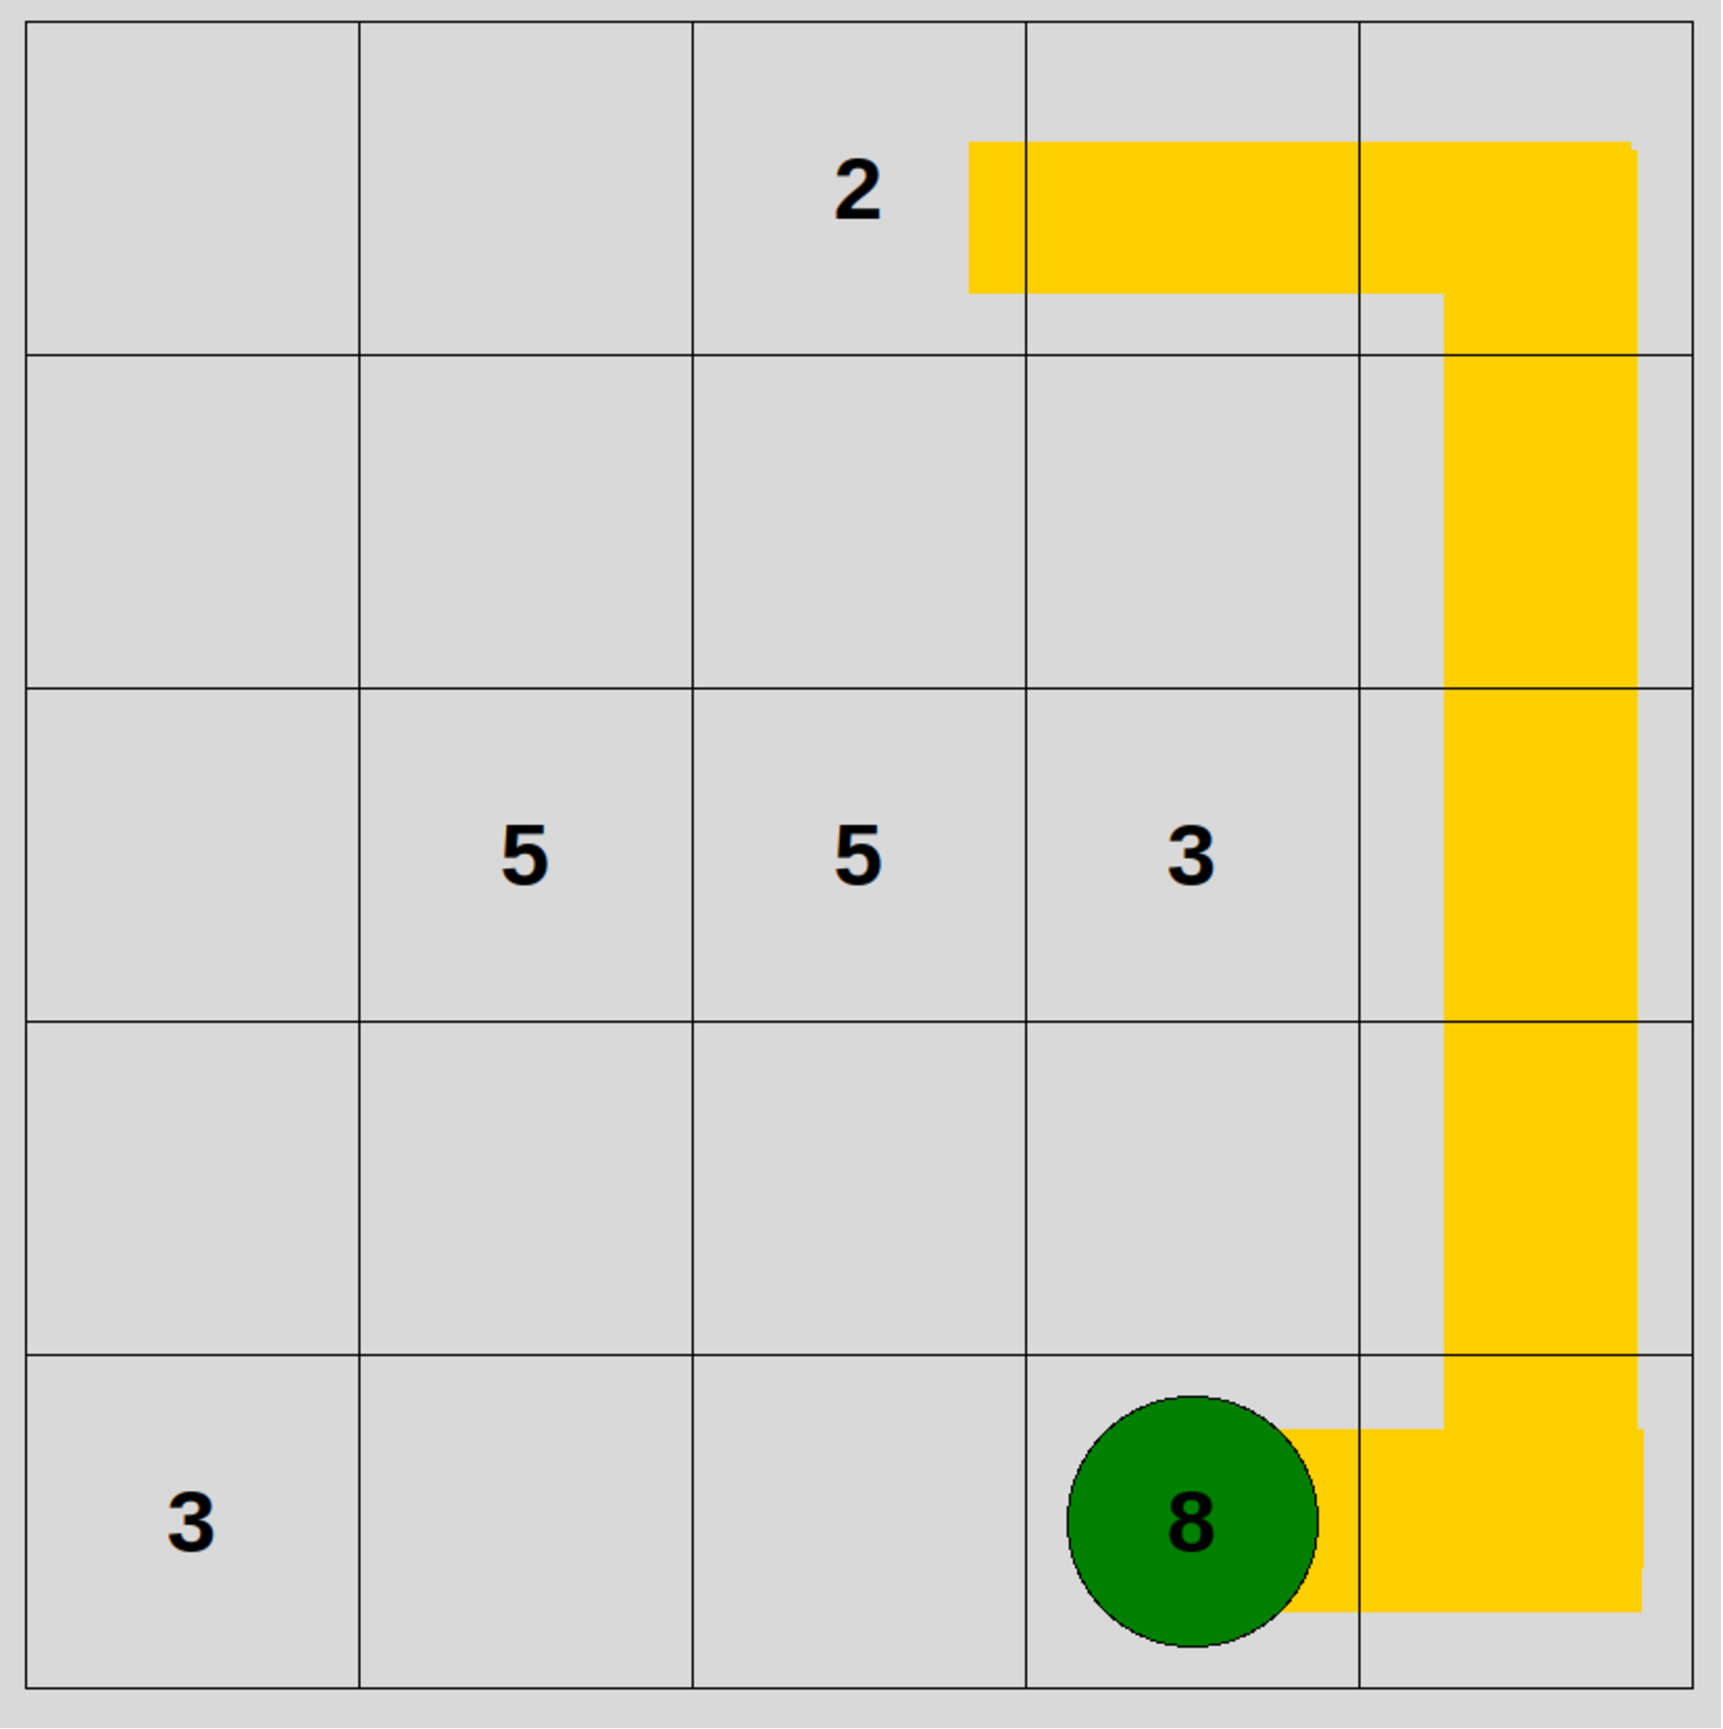
\includegraphics[width=0.25\textwidth]{shortest_w.pdf}
    \vspace{-25pt}
    \caption{Kürzester-Weg}
    \label{fig:weg}
\vspace{-20pt}
\end{wrapfigure}
\captionsetup[figure]{name=Abbildung}
In Abbildung \ref{fig:weg}  sieht man den kürzesten Weg vom Roboter zur Ersatz-Batterie mit der Ladung 2. Der kürzeste Weg ist gelb gekennzeichnet. Der Roboter kann nicht den direkten Weg gehen, da die Ersatz-Batterien 5 und 3 den Weg versperren.

Manchmal ist es sinnvoll nicht den \textbf{kürzesten Weg} zu einer anderen Batterie zu gehen.
Es kann auch vorteilhaft sein einen längeren Weg zu laufen. Dabei kann man fast alle Wege um eine \textbf{gerade Zahl verlängern}, indem man hin und her läuft, eine Verlängerung um eine ungerade Zahl ist im Umkehrschluss dagegen unmöglich.
Wenn man einen Weg vom Roboter zu einer Ersatz-Batterie finden will, dann sind alle anderen Ersatz-Batterien Hindernisse, welche nicht begehbar sind.





\paragraph{Weg Verlängern}


In Abbildung \ref{fig:weg_verlangern} wird gezeigt, wie ein Weg verlängert werden kann.
\paragraph{Stromrallye Darstellungsform}
Die kleinen Zahlen im oberen Bereich der Spielfelder zeigen die Lösungsschritte.
Eine Zahl $x$ bedeutet, dass dieses Spielfeld beim $x$ten Schritt vom Roboter besucht wird.
Felder, welche keine Zahlen haben, werden nie besucht.
\\
\begin{figure}[h]
    \centering
    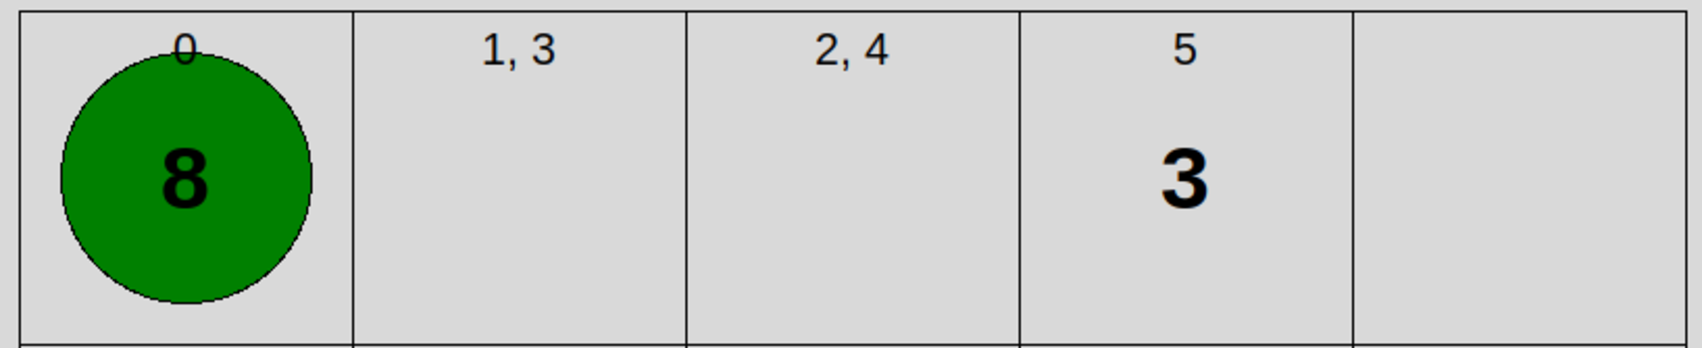
\includegraphics[height=0.09\textheight]{weg_verlaengern_n.pdf}
    \caption{Weg Verlangern}
    \label{fig:weg_verlangern}
\end{figure}
Diese Darstellungsform habe ich gewählt, da diese noch bei sehr komplexen Spielen leicht verständlich ist und es einfach war, ein Programm zu schreiben, welches diese generiert.
In diesem Beispiel ist der kürzeste Weg 3 Schritte lang, wurde aber auf 5 Schritte verlängert. Der Weg kann auch weiter verlängert werden, indem noch öfter hin und her gelaufen wird.

\par
Die \textbf{Kürzesten Wege} vom Roboter zu den anderen Batterien werden durch die \textbf{Breiten Suche} \cite{cormenBFS} herausgefunden, dies ist \textbf{A-Stern} \cite{hart} vorzuziehen, da dem Algorithmus A-Stern nur den Weg von einem Knoten zu einem anderen berechnet, die Breiten Suche findet bei einer Durchführung den kürzesten Weg zu allen anderen Knoten. Auch der \textbf{Djikstra} \cite{dijkstra} Algorithmus findet nach einer Durchführung den kürzesten Weg zu allen Knoten. \textbf{Breiten Suche} ist trotzdem die beste Wahl, da \textbf{Breiten Suche} die \textbf{Zeitkomplexität}, $E$ = Kanten; $V$ = Knoten $O(E + V)$ und \textbf{Djikstra} $O(V * log(V) + E)$ (wenn Djikstra mit Fibonacci-Heap verwendet wird) hat. Somit ist die \textbf{Breiten Suche schneller als Djikstra}.

\paragraph{Der Graph}
\captionsetup[figure]{name=Abb.}
\begin{wrapfigure}{r}{0.3\textwidth}
    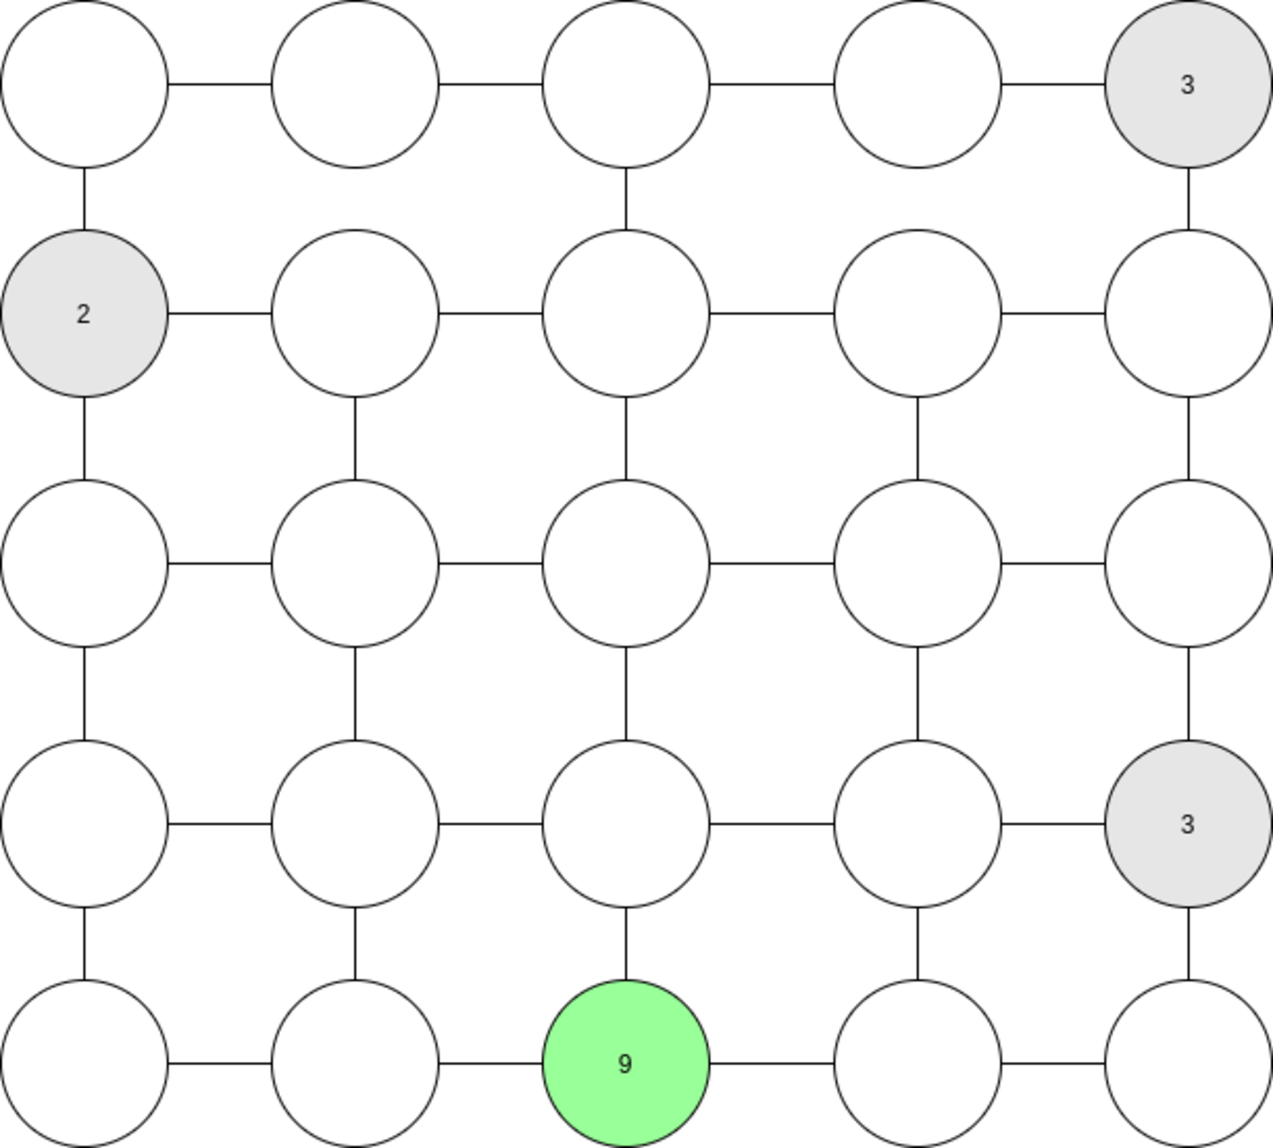
\includegraphics[width=0.3\textwidth]{graph_stromrallye.pdf}
    \caption{Das Stromrallye Spiel als Graph}
    \label{fig:graph_stromrallye}
    \vspace{-5pt}
\end{wrapfigure}
\captionsetup[figure]{name=Abbildung}
Man kann das Spielfeld in einen Graphen umwandeln, dabei sind die Spielfelder die Knoten.


Es handelt sich um einen ungerichteten, ungewichteten Graphen, alle Konten sind in beide Richtungen begehbar und haben das Gewicht 1.

Wenn man versucht den kürzesten Weg vom Roboter zu einer Batterie zu finden, sind alle anderen Batterien Hindernisse, da man eine Batterie aufnehmen muss, wenn man auf ihr Feld geht. Deswegen sind im erzeugten Graph alle Felder mit Batterien, außer der Ziel-Batterie, nicht begehbar.

In Abbildung \ref{fig:graph_stromrallye} sind zum besseren Verständnis die Ersatzbatterien in grau gekennzeichnet, der Roboter in grün.

In unserem Graphen, wird nicht gespeichert, wie groß die Ladung der Ersatzbatterien ist, dies ist in der Grafik nur für ein besseres Verständnis so dargestellt.
Der Graph speichert aber, ob ein Feld (dies entspricht im Graphen einem Knoten) begehbar ist. Ersatzbatterien sind nicht begehbar, wenn man den Weg zu einer anderen Batterie finden will.

\subsubsection{Erklärung Graph}
\begin{wrapfigure}{r}{0.5\textwidth}
    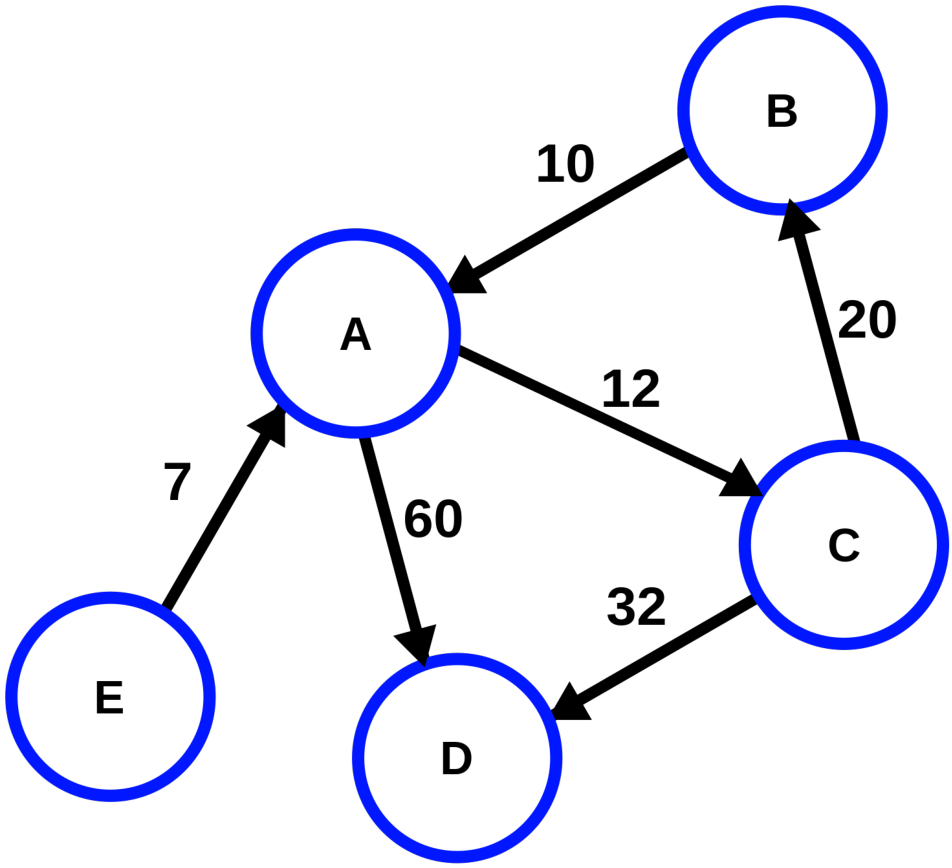
\includegraphics[width=0.5\textwidth]{graph.pdf}
    \caption{Ein Graph \textcite{wikipediaGraph}}
    \label{fig:graph}
\end{wrapfigure}
Ein Graph ist eine Datenstruktur und besteht aus Knoten und Kanten, wobei die Knoten  mit den Kanten verbunden sind (\textit{\textcite{biggs1986graph})}.
Es werden gerichtete und ungerichtete Graphen unterschieden.
In gerichteten Graphen haben Kanten eine Richtung, in ungerichteten nicht.
Man kann von einem Knoten über eine Kante zu einem anderen Knoten kommen usw..
In einem gewichteten Graphen haben Kanten zusätzlich ein Gewicht. Dies bedeutet, das ein bestimmtes Gewicht (oder Kosten) verwendet wird, um von dem einen Knoten zum anderen zu kommen.\cite{west1996introduction}

Beispielsweise in einem U-Bahn Netz stehen die Stationen für die Knoten. Die Kanten sind U-Bahn-Strecken und die Kosten der Kanten geben die Fahrtdauer der Strecken an.
\begin{figure}[h]
    \centering
    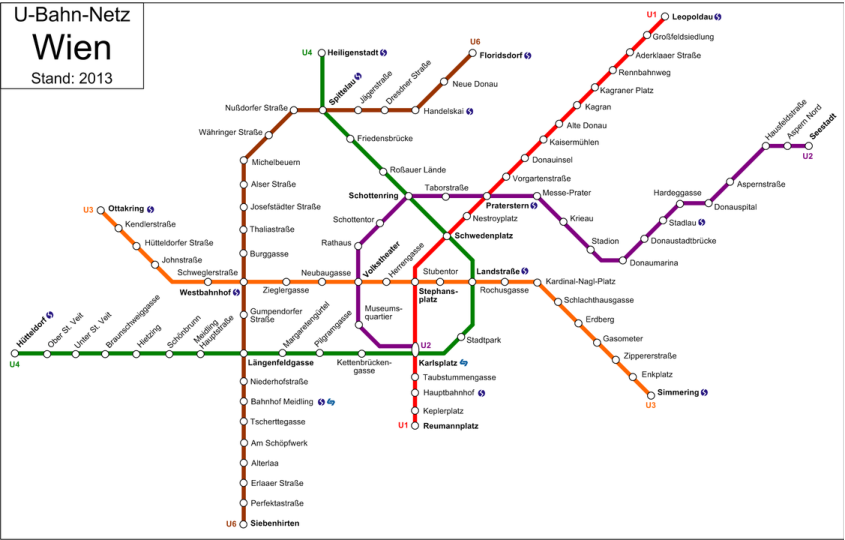
\includegraphics[width=0.5\textwidth]{u-bahn.pdf}
    \caption{Wiener U-bahn Netz \textcite{wikipediaUbahn}}
    \label{fig:u-bahn-netz}
\end{figure}



\subsubsection{Breiten Suche}


Bei der Breiten Suche startet man vom Startknoten und überprüft dann alle Kinder, bzw. Nachbarn des Startknotens, ob sie der Zielknoten (oder eines der Zielknoten) sind.
Dies wird veranschaulicht in der Abbildung .
Es folgt eine rekursive Durchführung für jeden Knoten.
In einem Set (Erklärung in Kapitel \ref{sec:HashSet}) wird gespeichert, welche Knoten bereits besucht worden sind und deswegen nicht nochmal besucht werden müssen.\cite{cormenBFS}
\par
Der Algorithmus terminiert, wenn entweder Wege zu allen Zielknoten gefunden oder alle Felder besucht worden sind (es kann sein, dass es zu einem Zielknoten gar keinen Weg gibt).

Die Breiten Suche funktioniert nur in einem Graph ohne Kanten Kosten, bzw. alle Kanten Kosten müssen gleich sein. In unserem Fall ist diese Bedingung gegeben, deswegen können wir die Breiten Suche verwenden, um den kürzesten Weg zu finden.
In unserem Graph hat jede Kante den Kosten 1, da der Roboter bei jedem Schritt eine Energieladung verbraucht.
\par
In unserem Fall kann die Breiten Suche auch bereits dann abgeschlossen werden, wenn alle Felder in der Reichweite des Roboters besucht wurden.

\begin{wrapfigure}{r}{0.3\textwidth}
    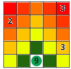
\includegraphics[width=0.3\textwidth]{Stromrallye_Feld_BFS.pdf}
    \caption{Spielfeld}
    \label{fig:bfs_stromrallye}
    \vspace{-20pt}
\end{wrapfigure}
\paragraph{In Abbildung \ref{fig:bfs_stromrallye}}
 sieht man eine durchgeführte Breiten Suche für das Stromrallye Spiel. Es werden die kürzesten Wege zu allen Feldern berechnet. Der kürzeste Weg zu einem Feld wird in der Abbildung, wie auch im Programm, gefunden, indem man vom Ziel-Feld zum Start geht und zwar so, dass die Farbe der abgelaufenen Felder sich von rot->leuchtrot->dunkel orange -> orange -> gelb -> grün verändert.
\setlength{\itemsep}{-60pt}
\\
Die Anzahl der Schritte zu einem Feld sind:
\small
\begin{compactitem}
\item 1 Schritt: grün
\item 2 Schritte: gelb
\item 3 Schritte: orange
\item 4 Schritte: dunkel orange
\item 5 Schritte: Leuchtrot
\item 6 Schritte: Rot
\end{compactitem}
\tiny{ \url{https://www.ralfarbpalette.de/ral-classic/ral-3024-leuchtrot}}  , \tiny{\url{https://www.99colors.net/color-names}}
\normalsize
\subsubsection{Djikstra}
Der Djikstra Algorithmus funktioniert ähnlich wie die Breiten Suche. Zusätzlich sortiert der Djikstra Algorithmus die Knoten nach Kosten und besucht zuerst den Knoten, zu dem ein Weg mit geringsten Kosten gefunden wurde. \cite{dijkstra}
\\
Dies bringt in unserem Fall nichts, da alle Knoten die gleichen Kosten haben und zwar 1.  Das Sortieren der Knoten macht allerdings den Djikstra Algorithmus langsamer  als die Breiten Suche.
\subsubsection{A-Stern}
 A-Stern nutzt eine zusätzliche Heuristik , um den bestmöglichen Pfad zuerst zu verwenden.
In unserem Fall wäre so eine Heuristik, wie weit der Knoten vom Zielknoten entfernt ist. 
Im A Stern Algorithmus werden dann Knoten, die näher am Zielknoten sind, zuerst besucht.
Dies macht den A Stern Algorithmus deutlich schneller als Djikstra und Breiten Suche.
Die Breiten Suche kann man durch die Verwendung einer Heuristik nochmal stark verbessern.
Da die Wahrscheinlichkeit, dass der schnellste Weg in der Richtung des Zielorts liegt, viel höher ist, wird dies bei  A Stern clever genutzt, um den Algorithmus wesentlich schneller zu machen. \cite{hart}

\subsubsection{Kürzester Weg-Fazit}


Die Breiten Suche ist am schnellsten, da diese mit einer Durchführung die kürzesten Wege zu allen Ziel-Knoten findet und außerdem keine zusätzliche Zeit durch Sortieren der Knoten verbraucht.



\par

\subsubsection{Kürzester Weg - Laufzeitanalyse}
In unserem ungerichteten Graphen ist der Weg von A nach B genauso lang und hat genau die gleichen Stationen (in umgekehrter Reihenfolge) wie der Weg von B nach A.
Damit die Breiten Suche nicht immer wieder neu ausgeführt wird, speichern wir unsere vorherigen Ergebnisse in einer HashMap. 
Der kürzeste Weg wird immer vom Roboter zu den Ersatzbatterien berechnet und er wird nur dann berechnet, wenn der Roboter auf einer Ersatzbatterie steht oder bei der Startposition.
Es gibt so viele Zielorte wie die \textbf{Anzahl-Ersatzbatterien}, außer wenn der Roboter sich beim Start schon auf einer Ersatzbatterie befindet, dann einer weniger.
Also wenn e die Anzahl der Ersatzbatterien ist, dann werden maximal
   \(\sum_{n=0}^{e} n\)  viele Wege berechnet.
Bei der Ausführung von Breiten Suche werden direkt von einem Start Wege zu allen Zielen gefunden. Deswegen muss die Breiten Suche maximal $e-1$ oft ausgeführt werden. Da die Breiten Suche $O(E+V)$ lange dauert, kommen wir so auf eine worst-case Laufzeitkomplexität von $O(e * (E + V))$.
\subsubsection{Sonderfälle}
\captionsetup[figure]{name=Abb.}
\begin{wrapfigure}{r}{0.3\textwidth}
    \vspace{-30pt}
    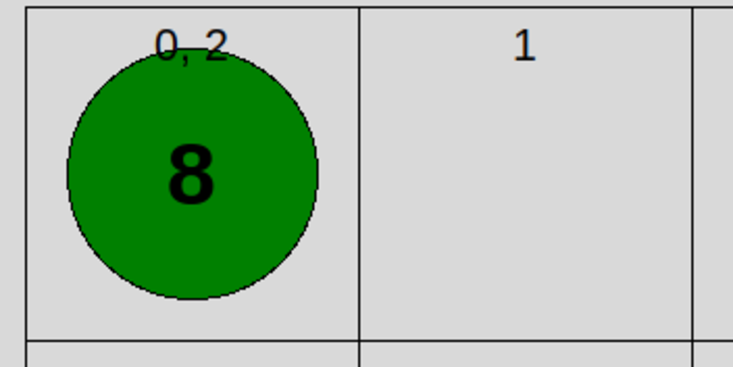
\includegraphics[width=0.3\textwidth]{way_to_self.pdf}
    \caption{Weg zu sich selbst}
    \label{fig:way_to_self}
    \vspace{-40pt}
\end{wrapfigure}
\captionsetup[figure]{name=Abbildung}
Von einer Ersatzbatterie kann es auch Sinn machen wieder zu sich selbst zu laufen, wobei der Weg zu sich selbst immer 2 Schritte lang ist. Es kann aber auch sein, dass es keinen Weg zu sich selbst gibt.
\captionsetup[figure]{name=Abb.}
\begin{wrapfigure}{l}{0.3\textwidth}
    \vspace{-20pt}
    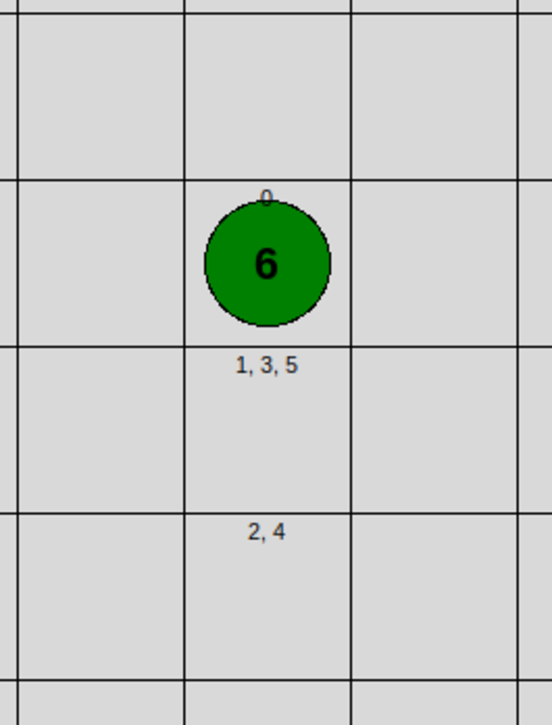
\includegraphics[width=0.3\textwidth]{way_ins_nothing.pdf}
    \caption{Weg ins nichts! Benutzung der ganzen Batterie-Ladung}
    \label{fig:way_to_nothing}
    \vspace{-20pt}
\end{wrapfigure}
\captionsetup[figure]{name=Abbildung}

Wenn alle Batterie-Ladungen 0 sind, nur der Roboter noch Ladung hat, muss dieser seine Ladung verlieren, indem er weitere Schritte läuft. Es kann aber vorkommen, dass dies nicht funktioniert, da alle Wege von anderen Batterien versperrt sind. Deswegen muss dies überprüft werden.

\subsubsection{Wege zu Ersatzbatterien}

Der \textbf{Roboter} kann von einer Position mit einem bestimmten Ladestand unterschiedliche Ersatzbatterien erreichen. Nachdem der Roboter zu einer dieser Ersatzbatterien gelaufen ist, kann dieser von dort wieder zu verschiedenen Ersatzbatterien laufen.
\par
Wie bereits beschrieben, kann es aber auch Sinn machen, dass der Roboter nicht den kürzesten Weg zu einer Ersatzbatterie geht. Da ein Weg immer um eine gerade Zahl verlängert werden kann, müssen diese Möglichkeiten auch durchgegangen werden.
Also wenn der kürzeste Weg $w$ lang ist und der Roboter $b$ Batterieladung hat. Die Reihe $a$ beinhaltet, alle möglichen Weglängen.
\[  a_1 = w \]
\[ a_{n+1} = x_{n} + 2  \{n \in \mathbb{N} | w + 2n < b\} \]
\paragraph{Zum Beispiel:}
Wenn der Roboter mindestens 5 Schritte zu einer Batterie braucht und gerade 9 Ladung hat, dann sind 5, 7, 9 mögliche Anzahl Schritte um zur Batterie zu kommen.
\\
Der kürzeste Weg ist 5 Schritte lang und der Roboter hat die Batterie-Ladung 9. Da der Weg um eine gerade Zahl verlängert werden kann, sind auch 7 und 9 möglich.

\subsubsection{Speicherung der Möglichkeiten}

Diese \textbf{Möglichkeiten} des Roboters werden in einem \textbf{Baum} gespeichert.
Dabei werden in den \textbf{Knoten} der Spielstand (Position und Ladestand der Ersatzbatterien und des Roboters) und in den \textbf{Kanten} die Schritte und Anzahl an Schritten, welche der Roboter laufen muss, um den Spielstand $a$ zu Spielstand $b$ zu verändern, angegeben.
Dabei ist Spielstand $b$ auch wieder ein Spiel welches gelöst werden kann.
\\
Um von Spielstand $a$ zu Spielstand $b$ zu kommen, muss der Roboter eine Schrittabfolge laufen.
Der Lösungsspielstand, besteht aus einem leeren Roboter und leeren Batterien.

\par
\subsubsection{Erklärung - Baum}
Ein Baum ist eine Art von Graph in welchem ein Knoten Kinder hat. Diese Kinder sind untereinander nicht verbunden.
Knoten haben immer nur einen Eltern-Knoten. Der Eltern-Knoten muss eine Ebene oben drüber sein. Die Kinder eines Knotens sind immer eine Ebene unten drunter.


\subsubsection{Lösung finden}
Um nun herauszufinden, ob es eine Lösung gibt und welche diese ist, wird der Weg mit der größten Anzahl an Schritten gesucht. Wenn die Anzahl der Schritte der Summe der Batterieladungen (der Ersatzbatterien und des Roboters) entspricht, ist dies eine korrekte Lösung um den Ladestand aller Batterien auf 0 zu bringen.
Abbildung:
%% TODO mit grün markiert!!!
Lösung mit grün markiert
\begin{itemize}
    \item RU : Batterie rechts unten auf dem Spiel
    \item RO: Batterie rechts oben auf dem Spiel
    \item LO: Batterie links oben
    \item RS: Roboters Startposition
\end{itemize}
\newpage

\begin{figure}[htpb]
    \centering
    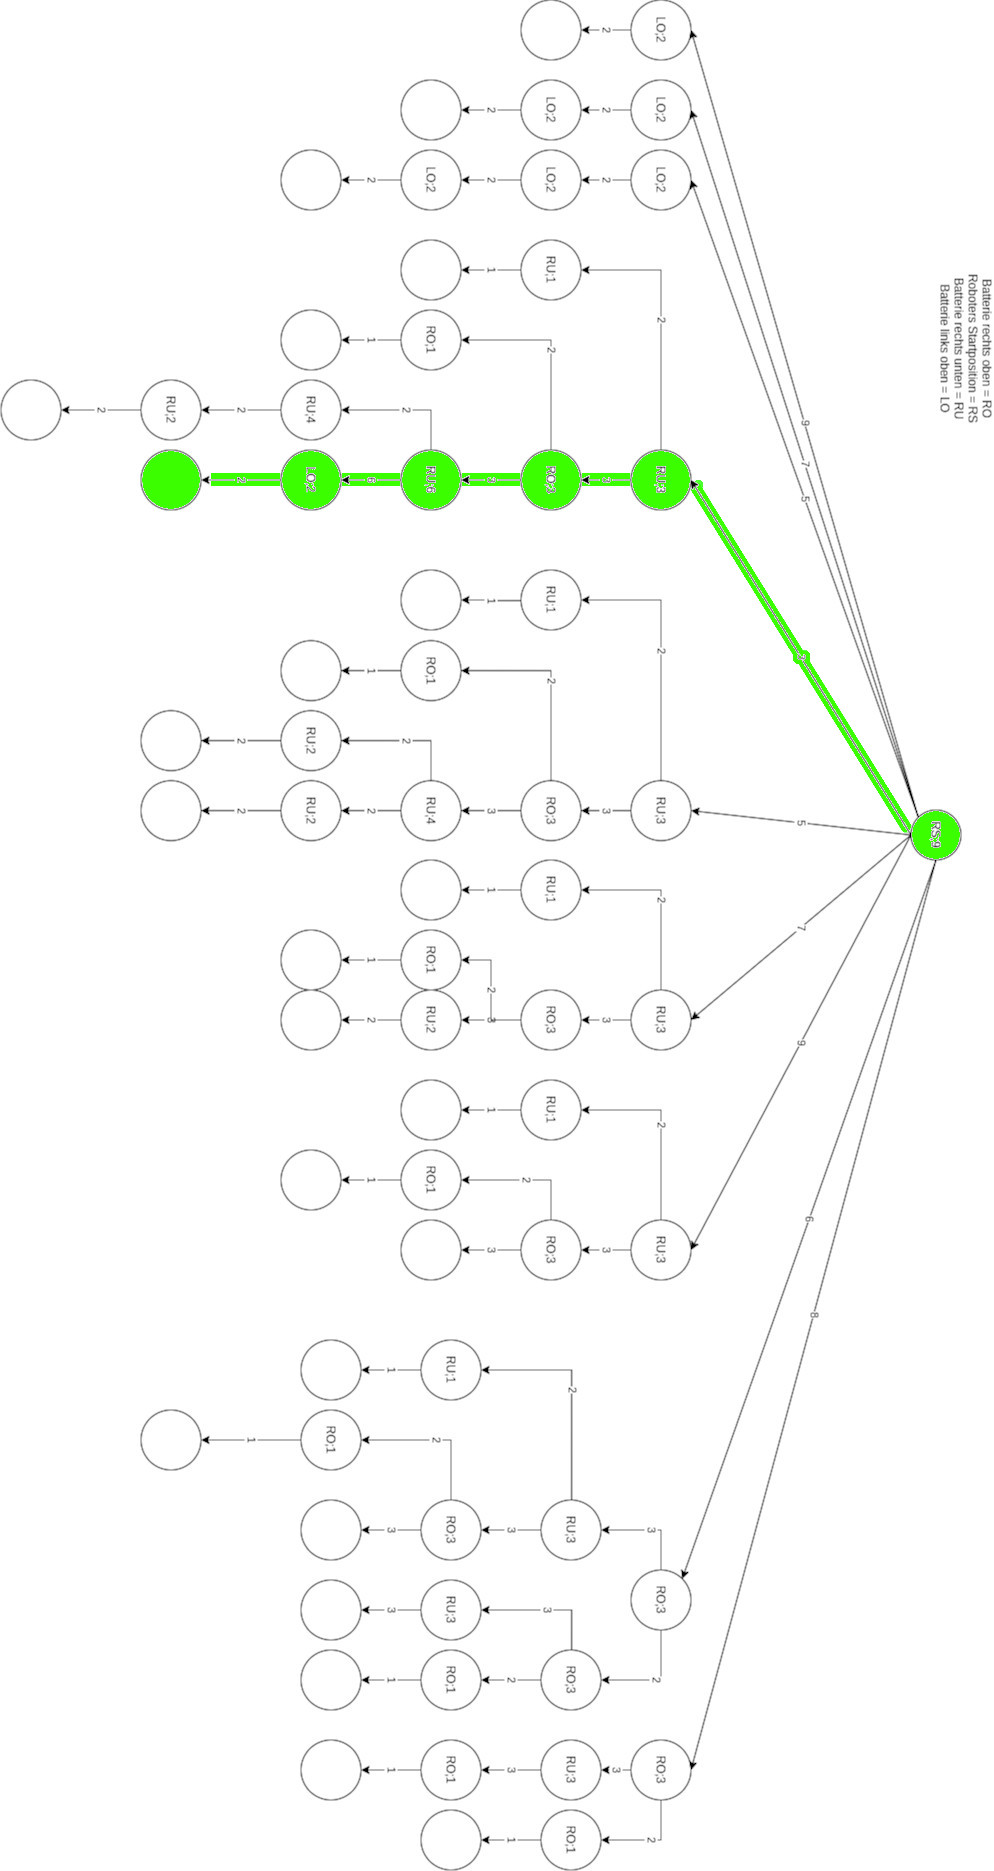
\includegraphics[height=0.9\textheight]{rotated_baum_v10.jpg}
    \caption{Schaubild des Moglichkeiten-Baums
    }
    \label{fig:moeglichkeiten_baum}
\end{figure}

\newpage

\subsubsection{Insgesamte Laufzeitanalyse}
Größen sind:
\begin{itemize}
    \item Größe des Spielfelds
    \item Anzahl Batterien
    \item Summe der Ladungen an Batterien
\end{itemize}

Die Laufzeit meines Algorithmus ist von all diesen genannten Größen abhängig.
Je größer das Spielfeld, je mehr Batterien und je mehr Ladung, desto länger braucht mein Programm.
Desto mehr Batterien, desto Länger braucht der Algorithmus.
Desto mehr Ladung, desto länger braucht mein Programm.
\par
Am abhängigsten ist mein Algorithmus, aber von der Anzahl an Batterien, da sich dadurch der Möglichkeiten-Baum sehr stark vergrößert, weil dann die Zahl an Knoten zunimmt.
\par
Der worst-case für meinen Algorithmus ist, dass sich auf jedem Feld des Spielfelds eine Batterie befindet, mit der Ladung 1. Dies führt zu einer Zeitkomplexität von $O(4)^L$; wenn $L$ die Gesamt Summe der Batterien ist, welche dann äquivalent zur Anzahl Felder ist, also der quadrierten Größe. Daher gilt auch $O(4^(s*s))$; $s$für size entspricht der Größe des Spielfelds.
Die 4, weil es 4 Richtungen gibt, in welche sich der Roboter bewegen kann.
\par
Die Zeit für das Berechnen der kürzesten Wege fällt bei Spielen mit vielen Batterien nicht so stark ins Gewicht.\par
Die Breiten Suche braucht $O(b * (E + V))$, $e$ Anzahl Ersatzbatterien, $E$ Edges, $V$ gleich Vertices. Jeder Knoten hat maximal 4 Kanten (bzw. Nachbarn), also $O(E) = O(V)$, $O(b * (E+V)) = O(b * V)$. In unserem worst-case Szenario, beschrieben im vorherigen Absatz, entspricht die Anzahl der Knoten, der Anzahl an Feldern, also $b=s*s$; $s$ für size ist die Größe des Spielfelds.
$V$ wiederum entspricht ebenfalls $s*s$. Daher kommen wir insgesamt auf $O(s*s*s*s)$,
also $O(s^4)$. Da $b$ = $s * s$. Können wir auch sagen $O(b^2)$. Also ist die Laufzeit der Breiten Suche quadratisch zur Anzahl Batterien.
Die Laufzeit für den Möglichkeiten-Baum ist wesentlich größer.
Sie ist $O(4^{(s*s)})$ oder $O(4^b)$.
Beide Laufzeiten addiert: $O(4^b) + O(b^2)$ = $O(4^b)$
\par
\textbf{Die insgesamte worst-case Laufzeit ist:}
\begin{compactitem}
\item In Abhängigkeit der Anzahl Batterien($b$) => \texttt{$O(4^e)$}
\item In Abhängigkeit der Größe des Spielfelds($s$) => \texttt{$O(4^{(s*s)})$}
\item In Abhängigkeit der gesamten Ladung(L)($L$) => \texttt{$O(4^L)$}
\end{compactitem}
\subsubsection{Umsetzung}
Der Algorithmus wird in Python (Version 3.7) implementiert.


\newpage
\subsubsection{UML-Klassen-Diagramm}
\begin{figure}[h]
    \centering
    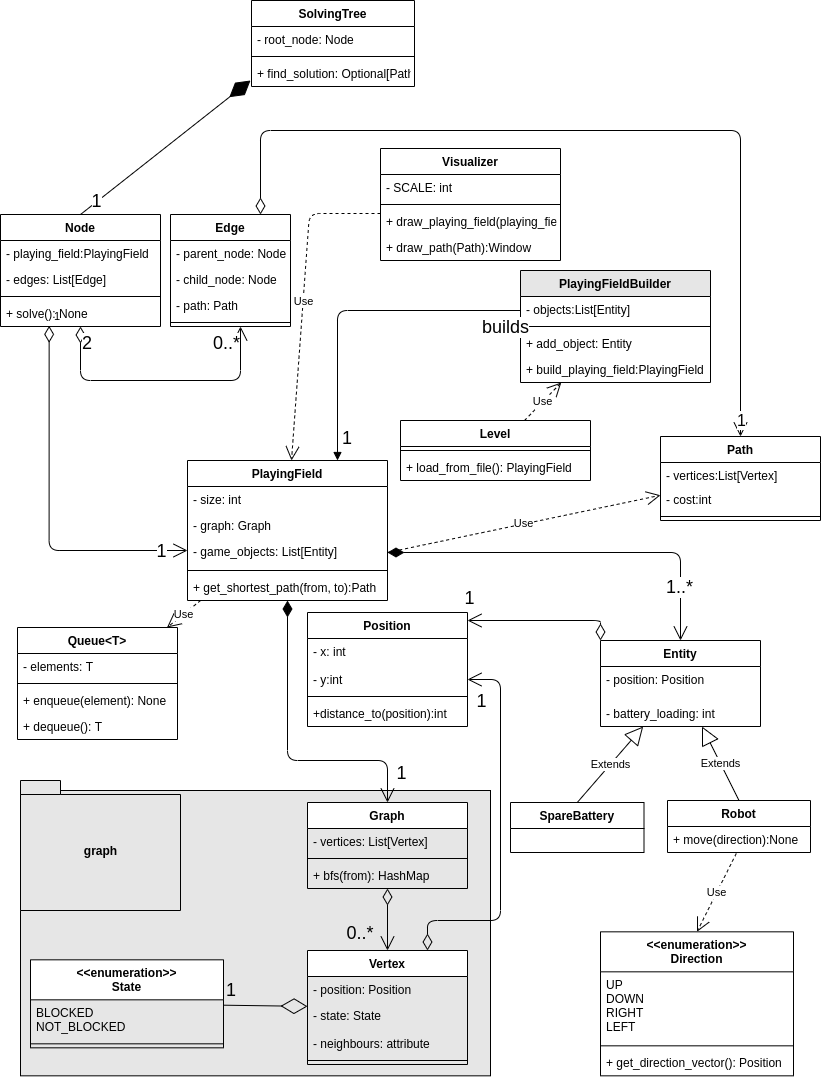
\includegraphics[width=0.85\textwidth]{uml_diagramm_v5.png}
    \caption{UML Klassen Diagramm}
    \label{fig:uml}
\end{figure}
\newpage

\newpage
\subsubsection{Lösungen}
\begin{wrapfigure}{l}{0.15\textwidth}
Eingabe:
\texttt{ \\
5 \\
3,5,9 \\
3 \\
5,1,3 \\
1,2,2 \\
5,4,3 \\
}
\end{wrapfigure}
\normalsize
Die Dateien enthalten jeweils ein Spielbrett mit den darauf verteilten Batterien und dem Roboter.
In der ersten Zeile ist Größe des Spielbretts angegeben, in der zweiten Zeile sind die Koordinaten des Roboters und die Ladung seiner Batterie und in der dritten Zeile ist die Anzahl der restlichen auf dem Spielbrett verteilten Batterien angegeben.
Ab der vierten Zeile ist in jeder Zeile eine Batterie angegeben, also ihre Koordinaten und ihre Ladung.
Dabei sind die Angaben zu den Koordinaten und der Ladung der Batterien und des Roboters als drei kommagetrennte Werte in der Form "x,y,ladung" geschrieben. \textcite{bwinfMaterial}.

\begin{wrapfigure}{l}{0.42\textwidth} 
    \vspace{-10pt}
    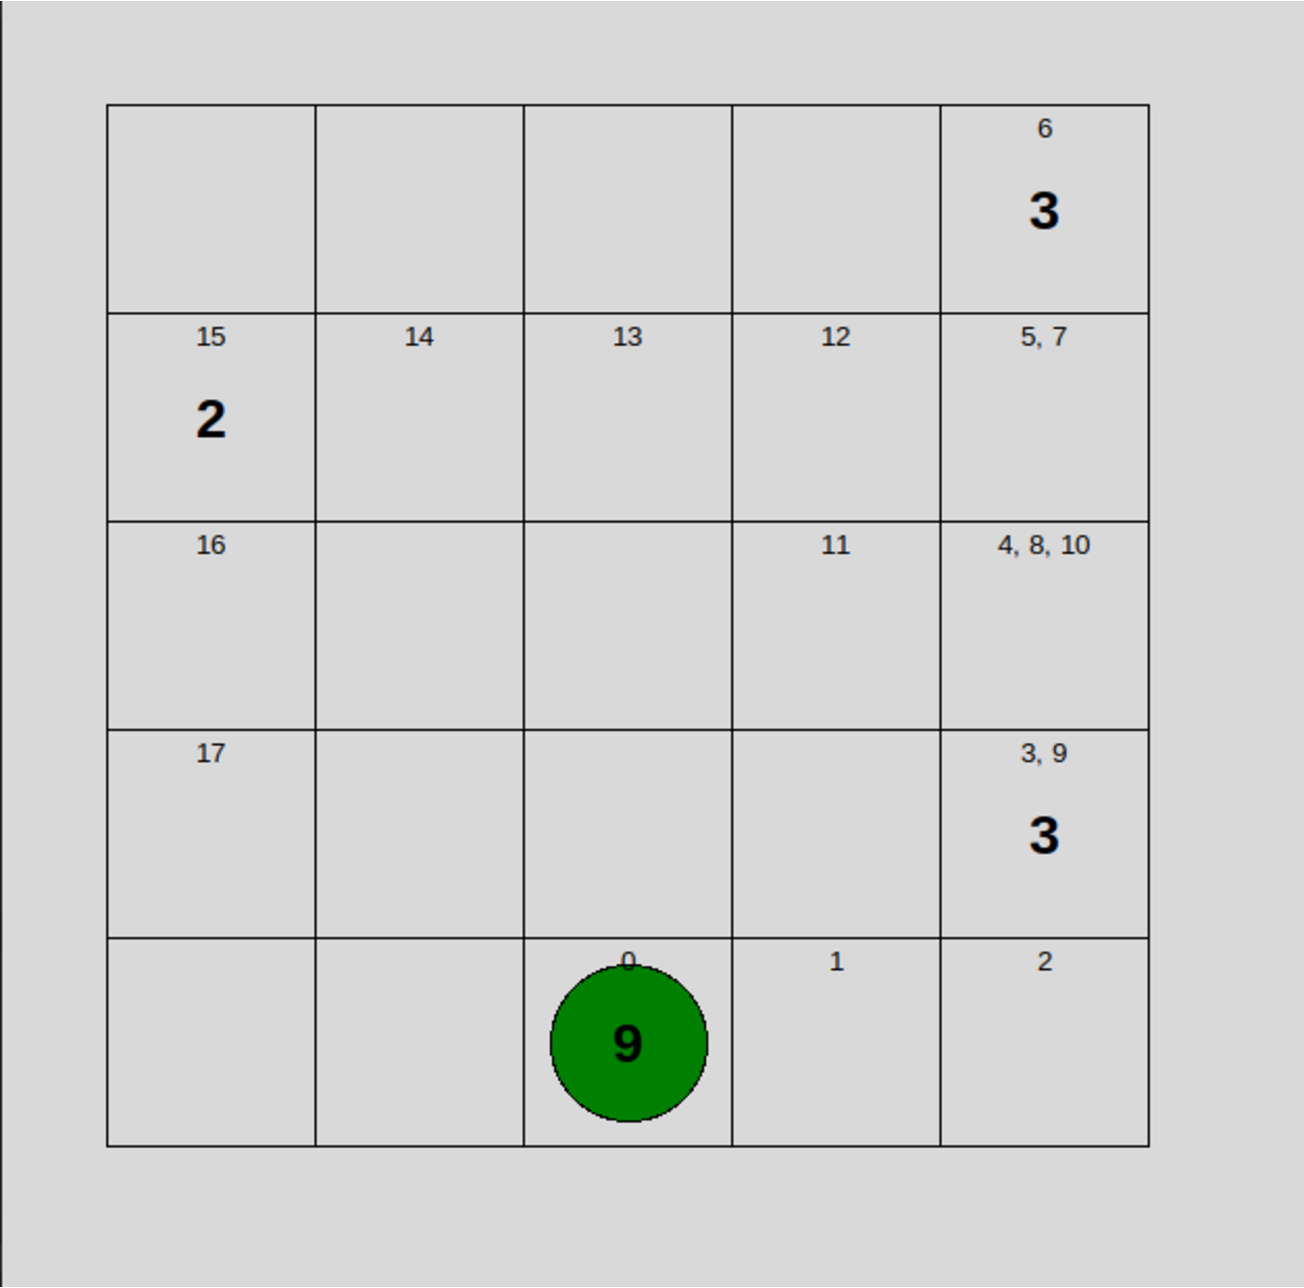
\includegraphics[width=0.4\textwidth]{Solution.pdf}
    \caption{Die Lösung des Stromrallye-Spiels}
    \label{fig:loesung1}
    \vspace{-35pt}
\end{wrapfigure}

In Abbildung \ref{fig:loesung1} sieht man die Lösung des BWinf Stromrallye Spiels. Die Zahl 9 mit dem grünen Kreis drumherum ist der Roboter, mit der Ladung 9.
Die Ersatzbatterien, sind die Fett gedruckten Zahlen in der Mitte der Felder, die Zahl zeigt die Ladung der Ersatzbatterien, beim Start an.
Die Ladung des Roboters und der Ersatzbatterien verändert sich während des Spiels, deswegen ist dies bloß eine Momentaufnahme beim Start des Spiels.
\\
Weitere Lösungen befinden sich im Anhang.
\\
\subsection{Aufgabe 1 b)}
\subsubsection{Beschreibung}
Bei Teil b) der Aufgabe 1 soll man selbst Stromrallye Spiele erstellen, welche lösbar sind, aber für einen Menschen schwer zu lösen.
(Siehe die Aufgabenstellung \ref{sec:aufgabenstellung} auf Seite\pageref{sec:aufgabenstellung})
\subsubsection{Lösungsidee}
Es werden zufällig Spielfelder generiert und dann mit dem Programm aus Aufgabe 1 a) geprüft, ob diese lösbar sind. Dabei werden an zufälligen Positionen Ersatz-Batterien mit einer zufälligen Ladung platziert. Die Position und die Ladung, des Roboters wird auch zufällig gewählt.
Die Größe des Spielfeld ist ebenfalls zufällig.
\subsubsection{Schwierigkeit des Spiels}
Das Spiel wird mit mehr Batterien deutlich schwerer zu lösen, auch ein größeres Spielfeld  macht es schwieriger.
\subsubsection{Lösung}
\begin{figure}[h]
    \centering
    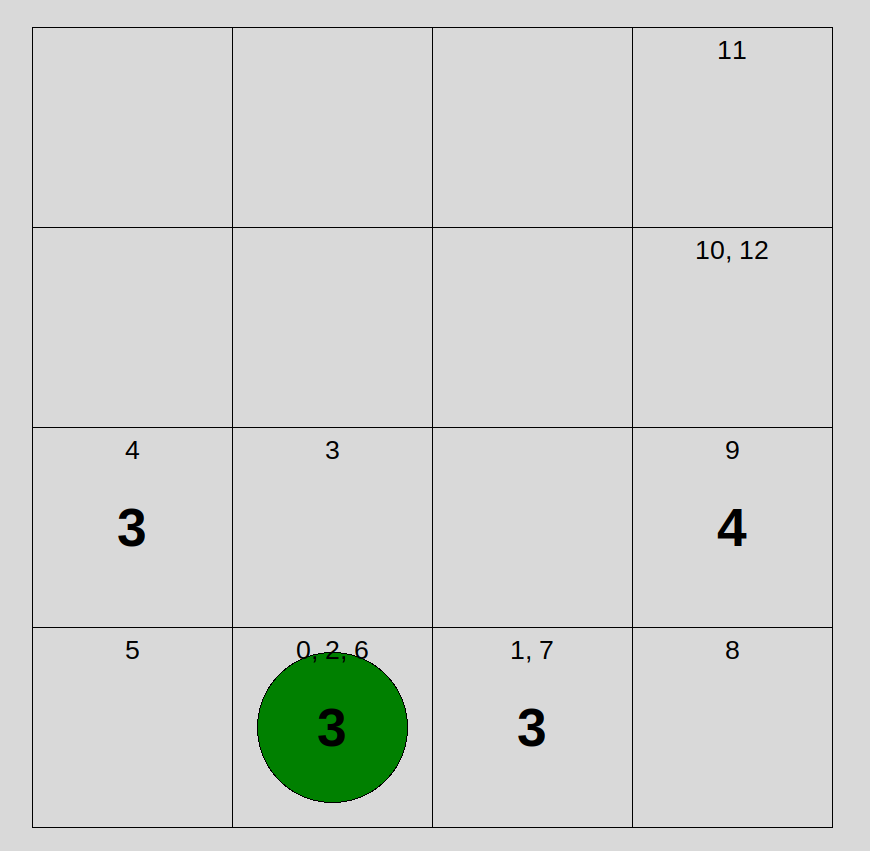
\includegraphics[width=0.5\textwidth]{aufgabe1_2_solution.png}
    \caption{Ein generisiertes Strom-Rallye Spiel}
    \label{fig:loesung2}
\end{figure}
\subsubsection{Umsetzung}
Die Informationen zur Umsetzung befinden sich im Anhang.

\subsection{Aufgabe 3}
\subsubsection{Aufgabenstellung}
Siehe im Anhang \ref{sec:aufgabenstellung} auf der Seite \pageref{sec:aufgabenstellung}.

\subsubsection{Lösungsidee}
\captionsetup[figure]{name=Abb.}
%%% da muss noch viel gemacht werden!!!
\begin{wrapfigure}{r}{0.3\textwidth}
    \vspace{-20pt}
    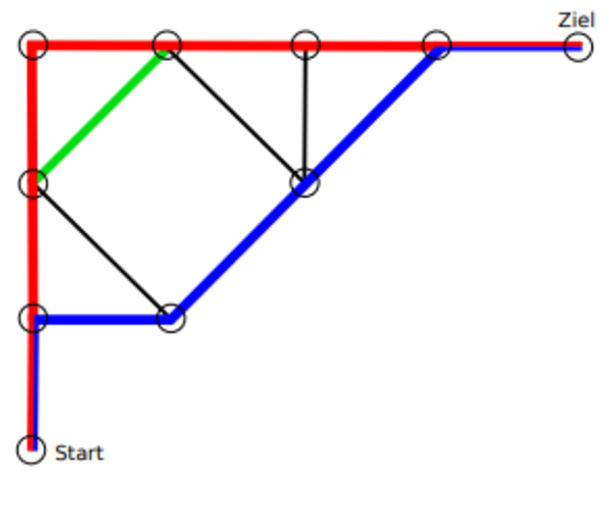
\includegraphics[width=0.3\textwidth]{aufgabe3.pdf}
    \caption{Straßennetz, rot ist der Weg mit den wenigsten Abkürzungen}
    \label{fig:abbiegen}
\end{wrapfigure}
\captionsetup[figure]{name=Abbildung}
Zunächst wandele ich das Straßennetz in einen Graphen um. Dabei werden
Straßenkreuzungen zu Knoten,  Straßen zu  Kanten und die Weglängen zu Kosten der Kanten.

\par
Dann finde ich in diesem Graphen alle möglichen Wege vom Start zum Ziel, allerdings nur Wege ohne Zyklen, also Wege, welche einen Knoten maximal 1 mal besuchen, da alle anderen Wege länger sind.Außerdem würde es sonst unendliche viele mögliche Wege geben, was die Aufgabe unlösbar machen würde.

\begin{wrapfigure}{l}{0.3\textwidth}
    \centering
    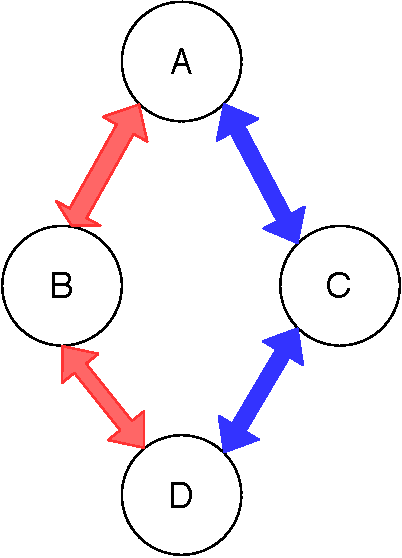
\includegraphics[width=0.3\textwidth]{small_example_graph.pdf}
    \caption{Graph}
    \label{fig:abbiegen}
    \vspace{-30pt}
\end{wrapfigure}
\par
Es gibt von A nach D, die möglichen Wege A -> B -> D und A -> C -> D.

\par
Um alle möglichen Wege zu finden, verwende ich die Tiefen Suche. Wenn man auf einen Knoten stößt, welcher das Ziel ist oder schon besucht wurde, wird abgebrochen.
\paragraph{Problem} Dieser Algorithmus braucht sehr lange, weil er alle Wege, die es in einem Graphen gibt, durch geht. An jeder Kreuzung gibt es  maximal 8 Straßen, da es Straßen nach oben, unten, rechts, links und diagonale  gibt.
Dies führt zu einer sehr schlechten worst-case Laufzeit von $O(8^V)$, V = Anzahl Kanten.
\paragraph{Verbesserung}
Die besten Pfade zu jedem Knoten (Kreuzung) werden in einer HashMap gespeichert. Am Anfang kennen wir nur den Weg zum Startknoten. Nun aktualisieren wir für alle Nachbarn des Startknotens die Map Einträge, dann von diesen Nachbarn wieder und so weiter.
Ein Knoten wird nur "betrachtet", wenn ein besserer Weg zu ihm gefunden wurde, also einer, der weniger Abbiegungen hat oder kürzer ist. So werden viel weniger Wege durchsucht.
\newpage
\begin{figure}[h]
    \centering
    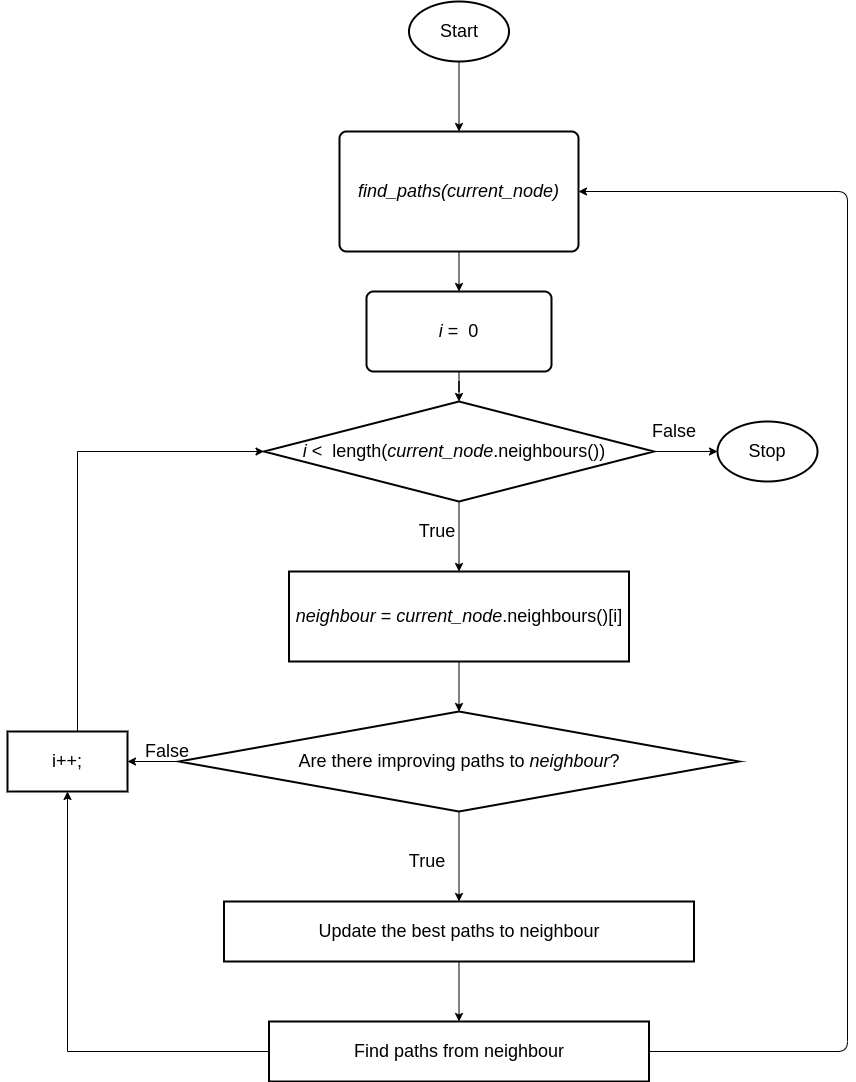
\includegraphics[width=0.9\textwidth]{pap_find_path_v4.png}
    \caption{Programmablaufplan um den besten Weg zu finden}
    \label{fig:pap3}
\end{figure}

\subsubsection{Abbiegungen bestimmen}

\begin{wrapfigure}{l}{0.4\textwidth}
    \centering
    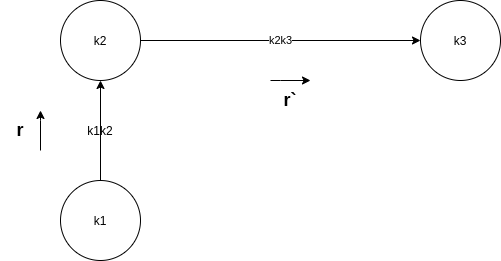
\includegraphics[width=0.4\textwidth]{AbbiegenBWinf.png}
    \caption{}
    \label{fig:abbiegen}
    \vspace{-30pt}
\end{wrapfigure}
Wenn man vom Knoten $k1$  zum Knoten $k2$ geht und beide eine Position $kp1$ und $kp2$ im 2-dimensionalen Raum haben, dann bewegt man sich in Richtung $r$ -> $r = kp2-kp1$ wenn man sich von  $k1$ zu $k2$  bewegt. Ebenso wenn man von $k2$ zu $k3$ geht, in Richtung $r'$-> $r' =kp3-kp2$. 
Wenn der Einheitsvektor $r^{0}$ von $r$ und der Einheitsvektor $r'^{0}$ von $r'$ ungleich sind handelt es sich um eine Abbiegung.
Wenn die Gleichung $r^0 \ne r'^0$ wahr ist, handelt es sich um eine Abbiegung.\\
Durch diese Definition lässt sich die Aufgabe auch für ein Straßennetz mit komplizierteren Kreuzungen durchführen.

\subsubsection{HashSet}\label{sec:HashSet}
Ein HashSet speichert eine Menge an Daten. Dabei hat es die besondere Eigenschaft, dass es keine Duplikate speichert, jedes Element ist entweder einmal oder kein mal enthalten.
Der Vorteil gegenüber einer Liste besteht darin, dass es nur $O(1)$ Zeit benötigt um zu prüfen, ob ein Element enthalten ist, sowie $O(1)$, um ein Element hinzuzufügen.
\cite{drohandata}

\subsubsection{HashMap}
Eine HashMap speichert key-value Paare, (auch HashTable genannt). Man kann für einen Schlüssel(key) einen entsprechenden Wert finden. Neue Key value Paare können in die HashMap eingetragen werden.
Um in einer Hashmap für einen Schlüssel einen Wert zu finden oder ein Wert-Schlüssel Paar einzufügen, wird nur konstante Zeit benötigt.
\cite{hashMap}

\section{Fazit}
In die Bearbeitung der beiden Aufgaben habe ich viel Zeit investiert. Obwohl beide Aufgaben an sich sehr unterschiedlich waren, konnte ich für beide Aufgaben ähnliche Algorithmen verwenden. Für beide Aufgaben war die Graphen-Theorie sehr hilfreich. Aufgrund der Seitenbeschränkung in der Facharbeit habe ich mich entschieden, die erste Aufgabe detailliert zu dokumentieren, um die Komplexität und die Vielzahl an Entscheidungen und Überlegungen, die in der Lösung der Aufgabe stecken, zu verdeutlichen. Die 3. Aufgabe konnte ich  nicht im gleichen Umfang wie die erste erklären, aber natürlich sind auch hier weitere Lösungen möglich und ähnliche Überlegungen zur Laufzeitoptimierung wie bei der ersten Aufgabe zu berücksichtigen.  
\section{Anhang}
\subsection{Offizielle Aufgabenbeschreibung des BWinf}
\cite{bwinfSpielfeld}
%\begin{figure}[h!]
%    \centering
%    \caption{Schaubild des Spielfelds mit Breiten Suche berechnete kürzeste Wege. grün: 1 Schritt, gelb: 2 Schritte -> \textcite{bwinfSpielfeld}}
%    \label{fig:bfs_stromrallye}
%\end{figure}

\label{sec:aufgabenstellung}
\includepdf[pages={4,6}]{aufgaben382.pdf}

\subsection{Programm Erklärung Aufgabe 1}
\begin{classInformation}{SolutionTree}
\addDescription{
Der \textit{SolutionTree} löst ein Spielfeld,
er speichert die \textit{root\_node} (siehe \ref{sec:Node} auf Seite \pageref{sec:Node}.)
Diese \textit{root\_node} hat wiederum Kind-Knoten, welche auch wieder Kind-Knoten haben usw. .
Mit der Funktion \textit{find\_solution} wird eine Lösung für das entsprechende Spielfeld (das Spielfeld wird nicht im \textit{SolutionTree} selbst gespeichert, aber in der \textit{root\_node} ) gefunden, falls eine existiert.}

\begin{relations}
\hasObjects{Node}{sec:Node}
\end{relations}


\begin{classAttributes}
\addAttribute{-}{root\_node}{Node}{Die \textit{root\_node} ist der oberste Knoten im \textit{SolutionTree}, sie hat selbst wieder Kind-Knoten welche wieder Kind-Knoten haben usw.}
\end{classAttributes}

\begin{classMethods}
\addMethod{+}{find\_solution()}{Optional[Path]}{Die \textit{find\_solution} Methode findet einen Pfad, welcher das Spielfeld, der \textit{root\_node} löst, falls es lösbar ist.}
\end{classMethods}
\end{classInformation}

\begin{classInformation}{Node}
\addDescription{Die \textit{Node}-Klasse ist Teil des \textit{Solution Tree} (siehe \ref{sec:SolutionTree} auf Seite \pageref{sec:SolutionTree}) . Außerdem speichert sie einen Spielstand des Stromrallye. Die \textit{Node} hat Kanten zu allen möglichen Knoten mit Spielständen, welche durch das Bewegen vom Roboter zu einer Ersatzbatterie möglich sind.}
\begin{relations}
\item ist Teil vom \textit{SolutionTree} (siehe \ref{sec:SolutionTree} auf Seite \pageref{sec:SolutionTree})
\hasObjects{Edge}{sec:Edge}
\hasObjects{PlayingField}{sec:PlayingField}
\end{relations}
\newpage
\begin{classAttributes}
\addAttribute{-}{edges}{List[Edge]}{Die \textit{edges} sind die Kanten zu den Kind-Knoten der \textit{Node} (siehe \ref{sec:Edge} auf Seite \pageref{sec:Edge})}.
\addAttribute{-}{playing\_field}{PlayingField}{Das \textit{playing\_field} ist der Spielstand dieses Knotens.}
\end{classAttributes}


\begin{classMethods}
\addMethod{+}{solve()}{None}
{
Die \textit{solve()} Funktion, löst den Spielstand des Knotens (\textit{playing\_field}). Dabei ruft die \textit{solve} Funktion rekursiv, wieder solve für alle Kind-Knoten des Knotens auf (siehe Pseudocode).
}
\end{classMethods}
\end{classInformation}


\begin{classInformation}{Edge}
\addDescription{Die \textit{Edge} Klasse ist die Kante welche Knoten im \textit{SolutionTree}(siehe \ref{sec:SolutionTree} auf Seite \pageref{sec:SolutionTree}) miteinander verbindet.
Es wird der Pfad gespeichert, welcher der Roboter laufen muss um den Zustand des Spielfelds von Eltern- zu Kind-Knoten zu verändern.}
\begin{relations}
\item ist Teil des \textit{SolutionTrees}
\hasObjects{Node}{sec:Node}
\hasObjects{Path}{sec:Path}
\end{relations}

\begin{classAttributes}
\addAttribute{-}{path}{Path}{Die \textit{path}-Variable, gibt an, welcher Pfad der Roboter gehen muss um den Zustand des Spielfelds vom Eltern-Knotens-Spielstand zum Kind-Knotens-Spielstand zu verändern.}
\addAttribute{-}{parent\_node}{Node}{Die \textit{parent\_node}  speichert den Eltern-Knoten}
\addAttribute{-}{child\_node}{Node}{Die \textit{child\_node}  speichert den Kind-Knoten}
\end{classAttributes}
\noMethods
\end{classInformation}

\begin{classInformation}{Entity}


\addDescription{
Die \textit{Entity} Klasse, beinhaltet alle Dinge, welche Roboter und Ersatzbatterie gemeinsam haben.
Roboter und Ersatzbatterie erben beide von Entity.
Beide haben eine Position und einen Ladestand.
}
\begin{classAttributes}
\addAttribute{-}{position}{Position}{Die \textit{position} gibt die Position der Entity auf dem Spielfeld an}
\addAttribute{-}{battery\_-loading}{int}{Der aktuelle Batterie-Ladestand der Batterie}
\end{classAttributes}
\noMethods
\end{classInformation}

\begin{classInformation}{Position}
\addDescription{Die \textbf{Position} Klasse, speichert die Position der entitys (Roboter, Ersatzbatterien).
Da wir uns im 2-dimensionalen Raum befinden, besteht die Position aus x und y Koordinate, welche Attribute der Position Klasse sind.\\
Dabei habe ich ein Kordinatensystem gewählt, indem %TODO
oben links ist.
Nach unten steigt y, nach rechts steigt x.
Die Positions Klasse könnte man auch als Vektor bezeichnen.
Sie implementiert die gängigsten Vektor-Funktionen, darunter (plus, minus, Länge des Vektors, Multiplikation ...)  

}

\begin{classAttributes}
\addAttribute{-}{x}{int}{Die x-Koordinate der Position.}
\addAttribute{-}{y}{int}{Die y-Koordinate der Position.}
\end{classAttributes}

\begin{classMethods}
\addMethod{+}{manhattan\_-distance(other\_-position)}{int}{manhattan distanz zur anderen Position. Die Manhattan Distanz wird folgendermaßen berechnet, $|x1 - x2| + |y1 - y2|$.
}
\end{classMethods}

\end{classInformation}

\begin{classInformation}{Roboter}
\addDescription{Der Roboter erbt von der Entity Klasse.
Zusätzlich hat der Roboter aber noch Methoden um sich zu bewegen und um seine Batterie mit einer Ersatzbatterie auszutauschen.}
\\
\textbf{wichtige Attribute:}
\\
erbt die Attribute \textit{position} und \textit{battery\_loading} von \textit{Entity}

\begin{classMethods}
\addMethod{+}{move(direction)}{None}{Der Roboter kann sich bewegen.}
\addMethod{-}{change\_-battery()}{None}{Der Roboter wechselt die Batterie, mit der unter sich liegenden Ersatzbatterie. Die Methode ist \textit{privat} und wird vom Roboter aufgerufen, wenn er sich auf ein Feld mit einer Ersatzbatterie bewegt.}
\end{classMethods}
\end{classInformation}
\newpage
\begin{classInformation}{Enum-Directions}
\addDescription{Das Enum Description, gibt die vier Richtungen (oben, unten, rechts, links) an, in welche sich der Roboter auf dem Stromrallye-Spielfeld bewegen kann.}
Die 4 verschiedenen Werte, welcher das Enum Directions haben kann sind:
\textbf{Directions.UP}\\
\textbf{Directions.DOWN}\\
\textbf{Directions.LEFT}\\
\textbf{Directions.RIGHT}\\

\begin{classMethods}
\addMethod{+}{get\_direction\_-vector()}{Position}{Die Methode getdirectionvector gibt, den entsprechenden Richtungsvektor der Richtung zurück- UP => (0, -1)- DOWN => (0, 1)- RIGHT => (1, 0) - LEFT => (-1, 0).
In diesem Fall ist unsere Positions-Klasse, der Richtungsvektor
}
\end{classMethods}
\end{classInformation}
\begin{classInformation}{SpareBatterie}
\addDescription{Die Ersatzbatterie (SpareBattery) erbt von der Entity-Klasse. Da sie sich nicht bewegen kann und auch sonst nichts machen kann, hat diese keine besonderen Attribute oder Funktionen.}

\textbf{wichtige Attribute:}\\
erbt \textit{position}und \textit{battery\_loading} von \textit{Entity}
\noMethods
\end{classInformation}

\begin{classInformation}{Spielfeld}
\addDescription{Die Spielfeld Klasse beinhaltet alle Objekte des Spiels. Sie speichert die Elemente des Spiels. Außerdem auch das Spielfeld als Graphen. Sie hat eine Größe, da sie quadratisch ist, wird nicht zwischen Länge und Breite unterschieden.
}
\newpage
\begin{classAttributes}
\addAttribute{-}{size}{int}{Die Größe des Spielfelds}
\addAttribute{-}{game\_objects}{List[Entity]}{Die Liste aller Objekte, die auf dem Spielfeld sind.}

\end{classAttributes}
\begin{classMethods}
\addMethod{+}{get\_shortest\_-path(-from:Position, to:Position)}{Path}{Findet den kürzesten Weg auf dem Spielfeld von einer Position zu einer anderen, ohne andere Ersatzbatterien aufzusammeln außer des Ziels.}
\end{classMethods}

\end{classInformation}

\begin{classInformation}{Graph}
\addDescription{Die Graph Klasse, entspricht einem normalen Graphen in der Informatik. Es ist ein ungerichteter, ungewichteter Graph, weswegen es auch keine Kanten als Objekte gibt, auch keine Klasse, da alle Kanten Kosten 0 haben.
Stattdessen speichert jeder Knoten(Vertex), die Nachbar Knoten(Vertices).
Der Graph speichert alle Knoten in einer Liste.}

\begin{classAttributes}
\addAttribute{-}{vertices}{HashMap-[Position,- Vertex]}{Alle Knoten des Graphen werden in der HashMap \textit{vertices} gespeichert. Es wird eine HashMap verwendet, da man bei solcher nur konstante Zeit O(1) benötigt um ein Knoten an einem Punkt zu bekommen. Eine weitere Alternative ist ein 2-dimensionales Array, bei dem an Stelle vertices[x][y] -> der Knoten der Position x y ist.}
\end{classAttributes}
\begin{classMethods}
\addMethod{+}{bfs(from, to)}{HashMap[Vertex, Path]}{Führt die breiten Suche (engl. \textbf{b}readth \textbf{f}irst \textbf{s}earch) aus.}
\end{classMethods}
\end{classInformation}

\begin{classInformation}{Vertex}
\addDescription{Die Vertex-Klasse, ist ein Knoten des Graphen. Der Knoten kennt seine Nachbar Knoten und hat eine Position.}
\begin{classAttributes}
\addAttribute{-}{position}{Position}{Position auf dem Spielfeld.}
\addAttribute{-}{neighbours}{List[Vertex]}{Nachbarknoten}
\end{classAttributes}
\begin{classMethods}
\addAttribute{+}{add\_neighbour}{None}{Fügt einen Knoten als Nachbar hinzu.}
\end{classMethods}
\end{classInformation}

\subsection{Umsetzung Aufgbabe 1 b)}
Die Implementierung ist wie in Aufgabe 1 Teil a) in Python. Aus dem Grund, dass ich den Algorithmus aus Teil 1 nutze, habe ich nur eine Klasse benötigt und zwar \textbf{PlayingFieldGenerator}
\paragraph{PlayingFieldGenerator}
\addDescription{Die PlayingFieldGenerator- Klasse ist die einzige Klasse, des 2.Teils. Diese erzeugt ein zufälliges, lösbares Stromrallye Spiel}
\begin{classAttributes}
\addAttribute{-}{playing\_-field\_builder}{Playing-Field-Builder}{baut das Spielfeld}
\addAttribute{-}{positions\_-used}{HashSet-[Position]}{Speichert alle Positionen an welchen bereits ein Objekt ist, damit nicht zwei Objekte an einem Ort sind. Das HashSet eignet sich dafür, da es nur $O(1)$ Zeit benötigt.}
\end{classAttributes}

\begin{classMethods}
\addMethod{+}{create\_-solveable\_-playing\_field}{PlayingField}{Die Methode erzeugt ein lösbares Spielfeld}
\end{classMethods}

\subsection{Beispiel3}
\subsubsection{Eingabe}
\texttt{ \\
14 \\
3,5,9 \\
3 \\
6,4,4 \\
5,12,10 \\
6,2,5 \\
}
\normalsize
\subsubsection{Lösung}
\begin{figure}[h]
    \centering
    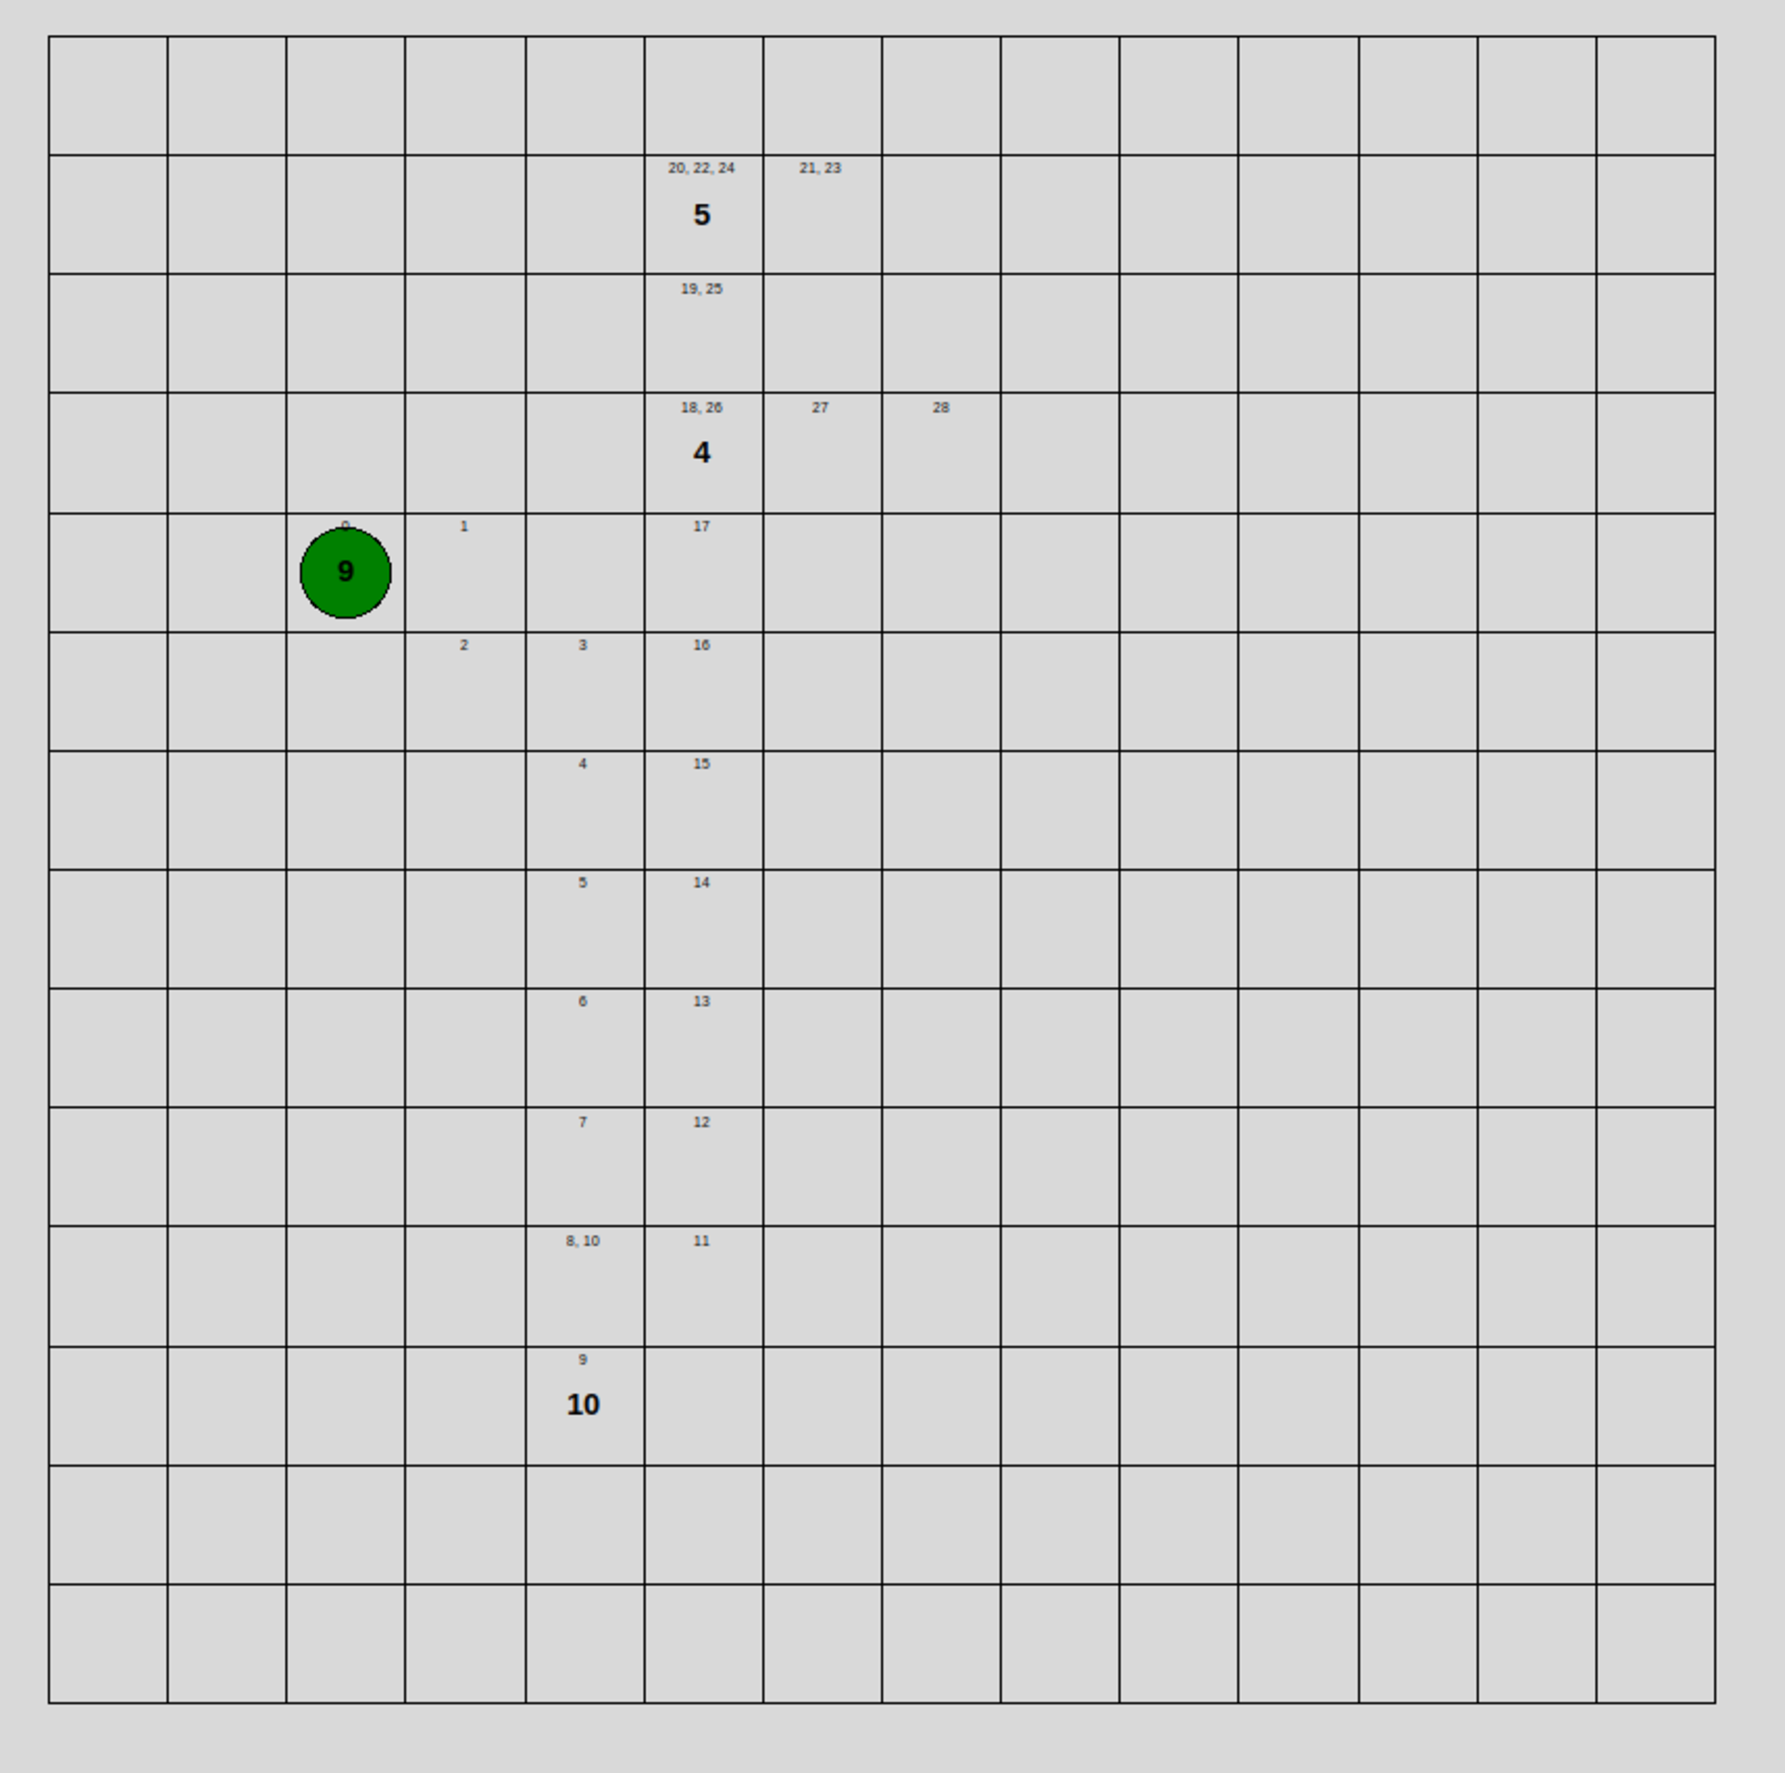
\includegraphics[width=0.5\textwidth]{solution3.pdf}
    \caption{Lösung des BWinfs Stromrallye Spiels Beispiel 3}
    \label{fig:loesung3}
\end{figure}

\subsection{Beispiel4}
\subsubsection{Eingabe}
\texttt{ \\
100 \\
40,25,20 \\
0 \\
}
\subsubsection{Lösung}
\begin{figure}[h]
    \centering
    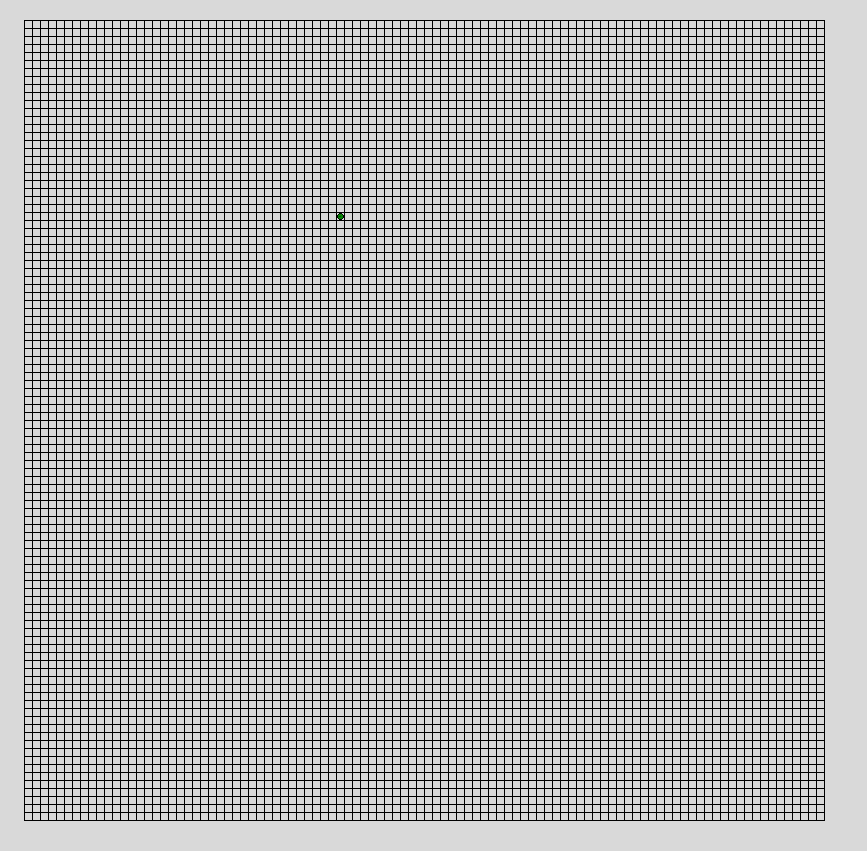
\includegraphics[width=0.5\textwidth]{solution4.png}
    \caption{Lösung des BWinfs Stromrallye Spiels Beispiel 4}
    \label{fig:loesung4}
\end{figure}
Da auf Grund der Größe wenig zu erkennen ist.
Hier heran gezoomt.
\begin{figure}[h]
    \centering
    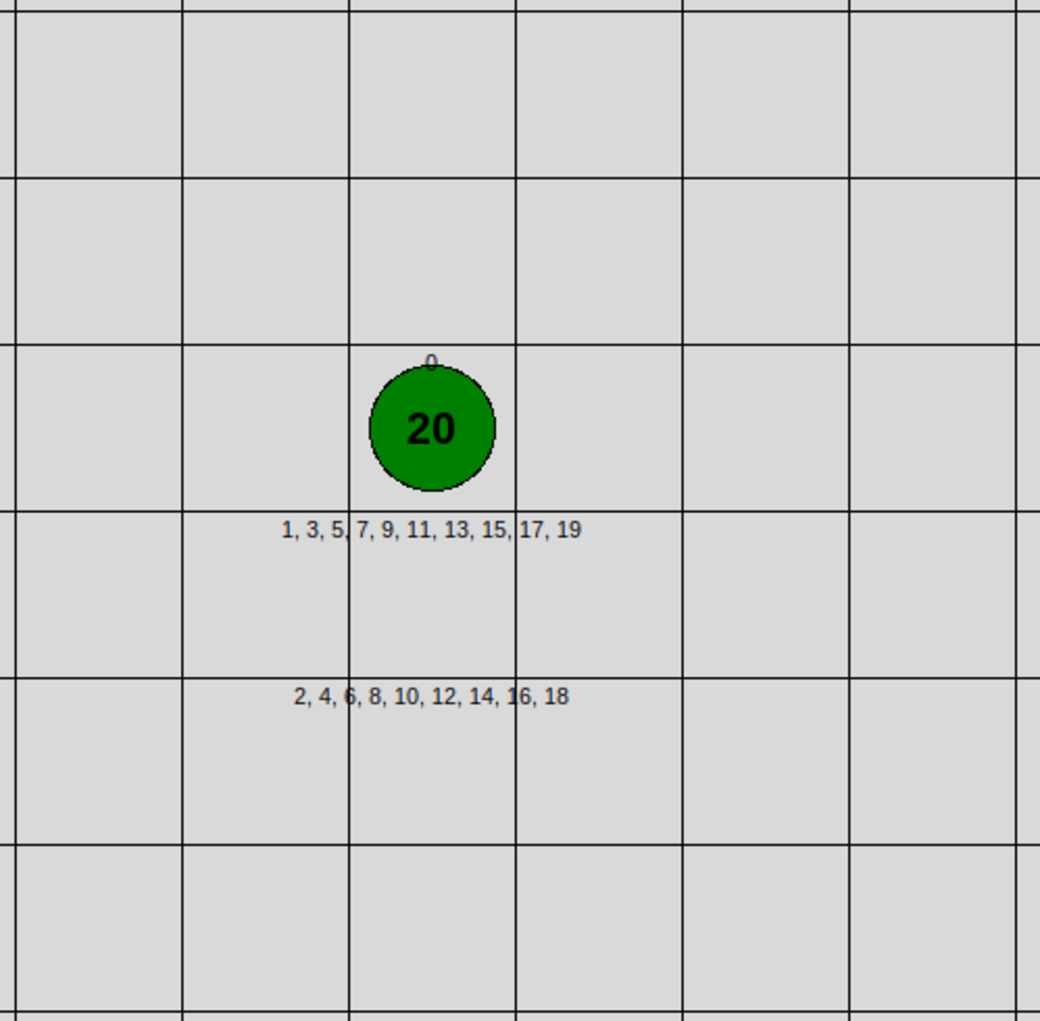
\includegraphics[width=0.4\textwidth]{solution_4_zoomed.pdf}
    \caption{Lösung des BWinfs Stromrallye Spiels Beispiel 4 heran gezoomt}
    \label{fig:loesung4_zoomed}
\end{figure}
\newpage

\section{Quellen}

\printbibheading
\printbibliography[omitnumbers=false,type=online,heading=subbibliography,title={Digital}]

%\subsection{Bücher}
%\newcommand{\addReference}[2]{\hspace{-25pt}[#1]\hspace{10pt} #2\par}
%\addReference{Ein25}{Einstein 2025 "Laura ist cool" S 5-8}
%\hspace{-10pt}\addReference{Ble20}{Laura Blechschmidt 2020 "Die Mikrowelle die Krebs heilt"  }

%\defbibenvironment{nolabelbib}
%  {\list
%     {[Ble20]}
%     {\setlength{\leftmargin}{\bibhang}%
%      \setlength{\itemindent}{-\leftmargin}%
%      \setlength{\itemsep}{\bibitemsep}%
%      \setlength{\parsep}{\bibparsep}}
%      }
%  {\endlist}
%  {\item}
  
\printbibliography[nottype=online, heading=subbibliography, title=Bücher]



\section{Erklärung über die selbständige Anfertigung der Arbeit}
Hiermit erkläre ich, dass ich die vorliegende Arbeit selbstständig und ohne fremde Hilfe verfasst, alle aus anderen Werken wörtlich oder sinngemäß entnommenen Stellen und Abbildungen unter Angabe der Quelle als Entlehnung kenntlich gemacht und keine anderen Hilfsmittel als die angegebenen verwendet habe. \\
\Ort, \today \space \Name


\end{document}
